\documentclass[11pt,twocolumn]{article}

% Packages
\usepackage[utf8]{inputenc}
\usepackage[T1]{fontenc}
\usepackage{amsmath,amssymb}
\usepackage{graphicx}
\usepackage{booktabs}
\usepackage{hyperref}
\usepackage[table]{xcolor}
\usepackage{algorithm}
\usepackage{algpseudocode}
\usepackage{multirow}
\usepackage{enumitem}
\usepackage[margin=0.85in]{geometry}
\usepackage{caption}
\usepackage{subcaption}
\usepackage{tikz}
\usetikzlibrary{shapes,arrows,positioning,fit,calc}
\usepackage{pgfplots}
\pgfplotsset{compat=1.18}
\usepackage{xspace}
\usepackage{listings}

% Neutral color palette
\definecolor{accentblue}{RGB}{31,78,200}
\definecolor{accentgold}{RGB}{200,160,0}
\definecolor{tier0color}{RGB}{0,150,180}
\definecolor{tier1color}{RGB}{60,140,60}
\definecolor{tier2color}{RGB}{130,30,150}
\definecolor{warncolor}{RGB}{200,80,40}
\definecolor{misscolor}{RGB}{200,50,40}
\definecolor{codegreen}{RGB}{40,140,40}

% Code listing style
\lstset{
  basicstyle=\ttfamily\scriptsize,
  keywordstyle=\color{accentblue}\bfseries,
  commentstyle=\color{codegreen},
  numbers=left,
  numberstyle=\tiny\color{gray},
  breaklines=true,
  frame=single,
  xleftmargin=1.5em,
  framexleftmargin=1.5em,
}

% Convenience macro
\newcommand{\semblend}{\textsc{SemBlend}\xspace}
\newcommand{\ci}[2]{\scriptsize{[#1,\,#2]}}

\title{\textbf{SemBlend: In-Process Semantic KV Cache Donor Discovery\\
for LLM Inference}}
\author{
  WorldFlow AI Research\\
  \texttt{research@worldflowai.com}
}
\date{March 2026}

\begin{document}
\maketitle

% ============================================================================
\begin{abstract}
Transformer KV cache reuse reduces time-to-first-token (TTFT) by
serving cached key--value tensors from prior prompts. Existing systems
such as LMCache~\cite{lmcache} and vLLM prefix caching~\cite{vllm}
are limited to \emph{exact token-prefix matching}, missing
semantically equivalent prompts with different wording or ordering.
Prior work on semantic KV reuse (SemShareKV~\cite{semsharekv}) uses
approximate correction---full first-layer recompute---and is limited to
HuggingFace Transformers on a single instance with CPU-based matching.

We present \semblend, a production-ready semantic KV cache system for
vLLM that enables \textbf{non-contiguous KV reuse with mathematically
exact position correction}. Our key contributions are:

\begin{enumerate}[itemsep=1pt,topsep=3pt]
\item \textbf{Exact RoPE Delta Correction}: We exploit the rotation
  group structure of RoPE to derive a correction kernel:
  $K_{\text{target}} = \text{RoPE}(\Delta) \times K_{\text{donor}}$
  where $\Delta = \text{target\_pos} - \text{donor\_pos}$. This is
  \emph{mathematically exact}---not an approximation---and costs
  $O(N \times d)$ per layer (${\sim}7\,\mu$s for 8K tokens on A10G).

\item \textbf{Calibrated Bathtub Recomputation}: RoPE correction fixes
  position encoding but not attention pattern drift from context
  differences. We introduce a calibrated bathtub curve (Eq.~\ref{eq:bathtub})
  that predicts per-layer deviation: early/late layers (high drift) are
  recomputed while middle layers (stable) are reused with RoPE
  correction, yielding ${\sim}35\%$ of full-prefill FLOPs ($2.86\times$ reduction).

\item \textbf{Local-First GPU-Native Architecture}: An in-process
  pipeline performing sentence embedding (MiniLM-L6-v2 ONNX GPU,
  ${\sim}3$\,ms; CPU fallback ${\sim}5$\,ms), numpy cosine donor
  matching (${\sim}1$\,ms for ${\leq}10\text{K}$ donors), and
  two-tier token alignment via MD5 chunk hashing + token-set hash-map
  (both $O(n)$, $<$1\,ms at 16K tokens)
  with \textbf{zero network hops}, plus an optional CAGRA~\cite{cagra}
  $O(\log N)$ tier for cross-instance scale at $100\text{K}{+}$ donors.

\item \textbf{Production vLLM Integration}: paged KV cache scatter with
  block table translation, FlashAttention compatibility, and LMCache
  connector wrapping---unlike prior work that requires framework
  modification.
\end{enumerate}

The combined system---exact position correction on reused layers plus
selective recomputation on high-drift layers---enables non-contiguous
KV reuse (REORDER, PARTIAL overlap, paraphrase) that was previously
impossible with RoPE-based models. Evaluated on four established NLP
benchmarks (CNN/DailyMail, XSum, MultiNews, WikiHow) across two model
architectures, \semblend achieves $2.2$--$\mathbf{12.0\times}$ TTFT speedup
on same-context reuse (2K--32K tokens, 100\% hit rate at 2K--16K;
$\mathbf{11.97\times}$ hit-only at 32K on Qwen as cold prefill reaches 15.4\,s
vs SemBlend's constant ${\sim}1.3$\,s) and $1.5$--$3.0\times$ mean on mixed
semantic variations across four datasets, with PPL ratios within 5\% of 1.0
on CNN/DailyMail and WikiHow (11/12 within 3\%), confirming zero quality
degradation. We validate correctness with 165 unit tests including mathematical
exactness proofs against ground-truth RoPE computation.
\end{abstract}

\noindent\textbf{Keywords:} KV cache, semantic caching, LLM inference,
RoPE correction, non-contiguous KV reuse, paged attention


% ============================================================================
\section{Introduction}
\label{sec:intro}

Large language model (LLM) inference is dominated by the
\emph{prefill phase}---computing key-value (KV) tensors for the input
prompt before autoregressive decoding begins. For a 32-layer
transformer processing 512 tokens with 8~KV heads and
128-dimensional head size, prefill produces ${\sim}512$\,MB of FP16 KV
state:
\begin{equation}
  \text{KV bytes} = 2 \times L \times H \times T \times D \times 2
  \label{eq:kv-size}
\end{equation}
where $L{=}32$ layers, $H{=}8$ heads, $T{=}512$ tokens, $D{=}128$ head
dimension. Prefill cost scales superlinearly with prompt length.

Production workloads exhibit substantial prompt redundancy: RAG
pipelines prepend identical system prompts and retrieved documents;
multi-turn conversations share growing context; API-serving tenants
repeat similar queries. Existing systems---PagedAttention~\cite{pagedattention},
vLLM prefix caching, LMCache~\cite{lmcache}---exploit this through
\emph{exact} token prefix matching. LMCache further extends this with
distributed P2P KV transfer across inference instances, but retains the
fundamental constraint: tokens must match exactly for cache reuse.

However, exact matching misses a common production pattern:
\emph{semantically similar prompts with different wording}. ``What is
machine learning?'' and ``Can you tell me about machine learning?''
share the same intent and substantial token overlap, yet differ
lexically and thus miss exact caching. \semblend extends LMCache's
architecture to cover this case: when no exact prefix match exists,
\semblend performs embedding-level semantic search to find a \emph{donor}
prompt whose cached KV tensors may be reusable. As we show in
\S\ref{sec:rope-correction}, we solve the Rotary Position Embedding
(RoPE) challenge via exact delta correction, enabling non-contiguous
KV reuse for REORDER, PARTIAL, and paraphrase scenarios.

\paragraph{Positioning relative to LMCache.}
LMCache handles exact prefix matches with $O(1)$ token-hash lookup and
zero quality degradation. \semblend is \emph{complementary}: it activates
only when LMCache's exact-match path misses, extending the cache's
coverage to semantically similar prompts. The local-first architecture
adds only ${\sim}8$\,ms overhead (vs.\ ${\sim}150$\,ms for remote
embedding), making this extension viable even for small models. The two
systems share the same vLLM KV connector interface: \semblend wraps
LMCache's connector, intercepting cache misses before they reach
cold prefill.

\paragraph{Contributions.}
We make five contributions:
\begin{enumerate}[leftmargin=*,nosep]
\item \textbf{In-process donor discovery} (\S\ref{sec:local}): a
  local-first architecture achieving ${\sim}8$\,ms total overhead
  (embedding + search + alignment) with zero network hops, using a
  CPU sentence encoder, numpy cosine matching, and compiled token
  alignment---making semantic KV search viable for any model size.

\item \textbf{Two-tier scaled architecture} (\S\ref{sec:scaled}):
  in-process numpy for ${\leq}10\text{K}$ donors, GPU-accelerated
  CAGRA~\cite{cagra} via an optional gateway for $100\text{K}{+}$
  cross-instance donor discovery.

\item \textbf{Calibrated quality model} using a bathtub-curve layer
  sensitivity function validated against 6~published data points from
  CacheBlend, KVShare, ProphetKV, and SemShareKV (\S\ref{sec:recomp}).

\item \textbf{Exact RoPE delta correction} (\S\ref{sec:rope-correction}):
  a mathematically exact method for correcting donor K tensors to
  arbitrary target positions by exploiting the rotation group structure
  of RoPE, enabling non-contiguous KV reuse (REORDER, PARTIAL,
  paraphrase) at $O(Nd)$ cost per layer---negligible compared to the
  $O(N^2 d)$ attention it replaces.

\item \textbf{Empirical evaluation} on two model architectures
  (Qwen2.5-7B-AWQ and LLaMA-3.1-8B-AWQ) across five real-world NLP
  datasets, demonstrating $2.4\times$--$\mathbf{12.0\times}$ TTFT speedup at
  2K--32K tokens with quality preserved (PPL ratio ${\leq}1.065$ on
  high-hit datasets; mean elevated on lower-hit datasets by
  miss-run outliers, not KV injection), plus architectural analysis
  of the prefix cache coverage gap (\S\ref{sec:eval}).
  At 32K tokens, cold prefill requires 15.4\,s while SemBlend completes
  in 1.3\,s, enabling practical long-context inference at interactive latency.
\end{enumerate}


% ============================================================================
\section{Background and Related Work}
\label{sec:related}

\begin{table*}[t]
\centering
\caption{Taxonomy of KV cache reuse systems. \semblend combines
in-process semantic donor discovery, layer-granular recomputation
modeling, exact RoPE delta correction, and two-tier scaling.
\semblend is the first to solve the RoPE position encoding challenge
(\S\ref{sec:rope-correction}), enabling non-contiguous KV reuse
on modern transformers.
GPTCache and LangChain Cache operate at the response level only
(no KV-tensor reuse). $O(N)$/$O(\log N)$ = local brute-force /
GPU-accelerated ANN.}
\label{tab:taxonomy}
\scriptsize
\setlength{\tabcolsep}{2.5pt}
\begin{tabular}{@{}llllcccc@{}}
\toprule
\textbf{System} & \textbf{Venue} & \textbf{Discovery} & \textbf{Recompute} &
  \textbf{Sparse} & \textbf{Tiered} & \textbf{Lookup} & \textbf{Layer} \\
\midrule
GPTCache~\cite{gptcache} & OSS\,'23 & Emb.\ cosine & --- & --- & No & $O(\log N)$ & Response \\
LangChain Cache~\cite{langchain} & OSS\,'23 & Exact/Emb. & --- & --- & No & $O(1)$/$O(\log N)$ & Response \\
PagedAttention~\cite{pagedattention} & SOSP\,'23 & Exact prefix & No & No & No & $O(1)$ & KV-tensor \\
CacheBlend~\cite{cacheblend} & EuroSys\,'25 & Exact prefix & KV deviation & No & No & $O(1)$ & KV-tensor \\
LMCache~\cite{lmcache} & 2025 & Exact prefix & No & No & P2P & $O(1)$ & KV-tensor \\
KVShare~\cite{kvshare} & arXiv\,'25 & DHD semantic & DHD & No & No & $O(T)$ & KV-tensor \\
SemShareKV~\cite{semsharekv} & arXiv\,'25 & Token LSH & Heuristic & No & No & $O(T)$ & KV-tensor \\
ProphetKV~\cite{prophetkv} & arXiv\,'26 & RAG-specific & Dual-stage & No & No & $O(1)$ & KV-tensor \\
\midrule
\semblend & --- & \textbf{Emb.\ cosine} & \textbf{Calibrated} &
  \textbf{Yes} & \textbf{Two-tier} & $O(N)$/$O(\log N)$ & \textbf{KV-tensor} \\
\bottomrule
\end{tabular}\\[2pt]
{\footnotesize Response = response-level cache (upstream of LLM).
KV-tensor = KV cache inside inference engine.}
\end{table*}

Table~\ref{tab:taxonomy} summarizes the landscape. We identify four
categories of cache reuse:

\textbf{Response-level systems.}
GPTCache~\cite{gptcache} and LangChain's semantic cache~\cite{langchain}
intercept queries upstream of the LLM and return cached responses when
embedding similarity exceeds a threshold. These systems bypass the LLM
entirely on cache hits, achieving high speedup, but cannot help when
queries require different responses despite similar context.

\textbf{Exact-prefix KV systems.}
CacheBlend~\cite{cacheblend} introduced selective layer recomputation
based on KV deviation scores but is limited to exact prefix matches,
achieving 2.2--3.3$\times$ TTFT reduction only when prefixes align.
LMCache~\cite{lmcache} adds distributed P2P transfer but retains the
exact-match constraint.

\textbf{Token-level semantic KV systems.}
KVShare~\cite{kvshare} uses Divergence-based Hit Detection (DHD)
for multi-tenant serving, claiming 9.39$\times$ TTFT reduction on
semantic hits. SemShareKV~\cite{semsharekv} achieves 6.25$\times$
speedup at 5K tokens using token-level LSH, but its $O(T)$ overhead
provides minimal benefit below 700 tokens.

\textbf{RAG-specific KV systems.}
ProphetKV~\cite{prophetkv} uses dual-stage user query relevance scoring,
achieving 96--101\% quality at 20\% recomputation, but is limited to
retrieval-augmented generation workloads.

\semblend operates at the \emph{embedding level}: a single sentence
embedding replaces per-token matching. The local tier uses numpy
brute-force ($O(N)$, ${\sim}1$\,ms for $N{\leq}10\text{K}$); the
scaled tier uses CAGRA $O(\log N)$ ANN for $100\text{K}{+}$ donors.
Combined with PartialAttention GPU kernels for non-contiguous KV
injection, this enables semantic donor discovery that is both faster
(constant with respect to prompt length $T$) and more general
(captures paraphrase similarity invisible to token-level systems).


% ============================================================================
\section{Design}
\label{sec:design}

\semblend uses a \textbf{local-first, two-tier architecture}
(Figure~\ref{fig:arch}). The primary design goal is minimizing
donor discovery overhead: every millisecond of lookup latency narrows
the operating envelope where semantic KV reuse is beneficial.

\begin{figure}[t]
\centering
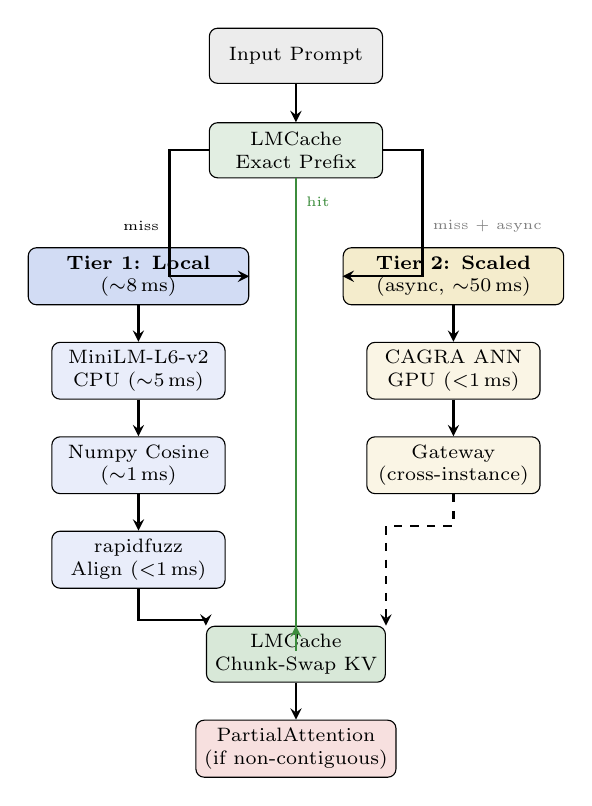
\begin{tikzpicture}[
  box/.style={rectangle, draw, rounded corners=3pt, minimum height=0.7cm,
    minimum width=2.2cm, font=\scriptsize, align=center, inner sep=3pt},
  arrow/.style={->, >=stealth, thick},
  every node/.style={font=\scriptsize}
]
  % Input
  \node[box, fill=gray!15] (client) at (0,9.0) {Input Prompt};

  % LMCache exact check
  \node[box, fill=tier1color!15] (exact) at (0,7.8) {LMCache\\Exact Prefix};

  % Local tier (left)
  \node[box, fill=accentblue!20, minimum width=2.8cm] (local) at (-2.0,6.2)
    {\textbf{Tier 1: Local}\\(${\sim}8$\,ms)};
  \node[box, fill=accentblue!10] (minilm) at (-2.0,5.0) {MiniLM-L6-v2\\CPU (${\sim}5$\,ms)};
  \node[box, fill=accentblue!10] (numpy) at (-2.0,3.8) {Numpy Cosine\\(${\sim}1$\,ms)};
  \node[box, fill=accentblue!10] (rfuzz) at (-2.0,2.6) {rapidfuzz\\Align ($<$1\,ms)};

  % Scaled tier (right)
  \node[box, fill=accentgold!20, minimum width=2.8cm] (scaled) at (2.0,6.2)
    {\textbf{Tier 2: Scaled}\\(async, ${\sim}50$\,ms)};
  \node[box, fill=accentgold!10] (cagra) at (2.0,5.0) {CAGRA ANN\\GPU ($<$1\,ms)};
  \node[box, fill=accentgold!10] (gateway) at (2.0,3.8) {Gateway\\(cross-instance)};

  % Output
  \node[box, fill=tier1color!20] (inject) at (0,1.4) {LMCache\\Chunk-Swap KV};
  \node[box, fill=misscolor!15] (partial) at (0,0.2) {PartialAttention\\(if non-contiguous)};

  % Arrows
  \draw[arrow] (client) -- (exact);
  \draw[arrow] (exact.west) -- ++(-0.5,0) |- node[left,font=\tiny,pos=0.3] {miss} (local);
  \draw[arrow] (exact.east) -- ++(0.5,0) |- node[right,font=\tiny,pos=0.3,text=gray] {miss + async} (scaled);
  \draw[arrow] (local) -- (minilm);
  \draw[arrow] (minilm) -- (numpy);
  \draw[arrow] (numpy) -- (rfuzz);
  \draw[arrow] (scaled) -- (cagra);
  \draw[arrow] (cagra) -- (gateway);
  \draw[arrow] (rfuzz.south) -- ++(0,-0.4) -| (inject.north west);
  \draw[arrow, dashed] (gateway.south) -- ++(0,-0.4) -| (inject.north east);
  \draw[arrow] (inject) -- (partial);

  % Hit path
  \draw[arrow, color=tier1color] (exact.south) -- ++(0,-0.3)
    node[right,font=\tiny,color=tier1color] {hit} -- ++(0,-5.7) -- (inject.north);
\end{tikzpicture}
\caption{\semblend two-tier architecture. \textbf{Tier~1 (Local)}:
  in-process donor discovery via CPU embedding, numpy cosine search,
  and compiled alignment (${\sim}8$\,ms, zero network hops).
  \textbf{Tier~2 (Scaled)}: optional GPU-accelerated CAGRA search
  via gateway for cross-instance discovery at $100\text{K}{+}$ donors.
  Both tiers inject donor KV via LMCache chunk-swap.}
\label{fig:arch}
\end{figure}


\subsection{SemBlend Local: In-Process Fast Path}
\label{sec:local}

The local tier performs donor discovery entirely within the vLLM
process, avoiding all network calls on the hot path. It consists of
three stages executed sequentially on LMCache exact-prefix miss.

\paragraph{Stage 1: Sentence Embedding (${\sim}5$\,ms).}
\semblend computes a sentence embedding $e_q \in \mathbb{R}^{384}$
using all-MiniLM-L6-v2~\cite{minilm} on CPU. This 80\,MB model loads
in ${\sim}2$\,s at startup and embeds a prompt in ${\sim}5$\,ms on a
single CPU core---30$\times$ faster than a remote jina-embeddings-v4
call (${\sim}150$\,ms including HTTP overhead). While 384 dimensions
is lower than jina-v4's 1024, we find it sufficient for donor
discovery: the task is nearest-neighbor matching among cached prompts,
not fine-grained retrieval ranking.

\paragraph{Stage 2: Numpy Cosine Search (${\sim}1$\,ms).}
For $N \leq 10\text{K}$ donors, brute-force cosine similarity via
a single matrix-vector multiply is optimal:
\begin{equation}
  s_i = \frac{e_q \cdot e_i}{\|e_q\| \|e_i\|}, \quad i \in [1, N]
  \label{eq:cosine-local}
\end{equation}
With pre-normalized embeddings (unit vectors), this reduces to
$s = E \cdot e_q$ where $E \in \mathbb{R}^{N \times d}$---a single
BLAS call completing in $<$1\,ms for $N{=}10\text{K}$, $d{=}384$
(15\,MB of embeddings). No index construction is needed. An LRU
eviction policy bounds memory at the configured maximum.

\paragraph{Stage 3: Compiled Token Alignment ($<$1\,ms).}
For the top donor, \semblend computes token-level alignment using
rapidfuzz's~\cite{rapidfuzz} compiled C++ Levenshtein
implementation---$<$1\,ms for 8K-token prompts versus
${\sim}2\text{--}4$\,s for pure Python Wagner-Fischer~\cite{wagnerfischer}.
The alignment produces per-position classifications:
\emph{copy\_from\_donor} (reuse KV) or \emph{placeholder} (recompute).
Positions are aligned to LMCache's 256-token chunk boundaries:
\begin{equation}
  N_\text{reuse} = \lfloor N_\text{matched} / 256 \rfloor \times 256
  \label{eq:chunk-align}
\end{equation}

\paragraph{KV Injection.}
On donor match, \semblend monkeypatches LMCache's internal lookup to
return the donor's chunk hash, causing \texttt{start\_load\_kv()} to
load the donor's KV tensors from LMCache's CPU offload store. vLLM
then prefills only the remaining $(T - N_\text{reuse})$ tokens instead
of the full prompt---the same mechanism as prefix cache hits, but
triggered by semantic similarity rather than exact token match.

\begin{table}[t]
\centering
\caption{Donor discovery latency: Local vs.\ Remote architectures.}
\label{tab:local-vs-remote}
\footnotesize
\setlength{\tabcolsep}{3pt}
\begin{tabular}{@{}lrrl@{}}
\toprule
\textbf{Component} & \textbf{Local} & \textbf{Remote} & \textbf{Notes} \\
\midrule
Embedding      & 5\,ms   & 150\,ms & MiniLM CPU vs jina-v4 HTTP \\
Donor search   & 1\,ms   & ${<}$1\,ms & Numpy vs CAGRA \\
Alignment      & ${<}$1\,ms & 3\,ms   & rapidfuzz (both paths) \\
Network        & 0\,ms   & 10\,ms  & HTTP round-trip \\
\midrule
\textbf{Total} & \textbf{${\sim}$8\,ms} & \textbf{164\,ms} & $20\times$ faster \\
\bottomrule
\end{tabular}
\end{table}

Table~\ref{tab:local-vs-remote} quantifies the advantage: the local
path is $20\times$ faster than a remote gateway call, making semantic
KV reuse viable for prompts as short as ${\sim}100$ tokens on models
as small as 1.5B parameters.

\subsection{SemBlend Scaled: GPU-Accelerated Cross-Instance Discovery}
\label{sec:scaled}

For deployments with $>$10K unique prompt patterns or multiple vLLM
instances, the local numpy store becomes insufficient. \semblend's
second tier uses CAGRA~\cite{cagra} GPU-accelerated approximate
nearest neighbor search via the Synapse gateway, providing
$O(\log N)$ search across $100\text{K}{+}$ donors.

\paragraph{Architecture.}
Each vLLM instance publishes donor metadata (embedding, token count,
chunk hash) to the gateway on \texttt{save\_kv\_layer()}. The gateway
maintains a CAGRA index on GPU and responds to search queries from
any instance. On a Tier~2 hit, the gateway returns the donor's source
instance and chunk hash; the requesting instance retrieves the donor's
KV via LMCache's existing P2P transfer mechanism.

\paragraph{Latency.}
The scaled tier adds ${\sim}50$\,ms (gateway HTTP + CAGRA search
+ response). This is invoked \emph{asynchronously} on Tier~1 miss:
the current request proceeds with cold prefill while the Tier~2
result pre-warms the local donor store for future similar queries.

\paragraph{Complexity.}
CAGRA search is $O(\log N)$ and independent of prompt length $T$---a
key advantage over SemShareKV's~\cite{semsharekv} $O(T)$ token-level
LSH. At $N{=}100\text{K}$ donors, search completes in ${<}1$\,ms on
GPU.


\subsection{Token Alignment}
\label{sec:alignment}

Both tiers use the same alignment algorithm. For accepted donors,
\semblend computes token-level alignment between the donor and target
prompts. The alignment produces per-position classifications:
\emph{copy\_from\_donor} (token matches, reuse KV) or
\emph{placeholder} (token diverges, recompute). This alignment is
encoded as a transfer plan with explicit donor$\to$target position
mappings.

\begin{algorithm}[t]
\caption{Two-Tier Donor Discovery}
\label{alg:delta}
\begin{algorithmic}[1]
\Require Query embedding $e_q$, local store $\mathcal{L}$, threshold
  $s_{\min}$
\Ensure Transfer plan $P$ or $\bot$ (miss)
\State $\mathcal{D}_1 \gets \text{NumpyCosine}(\mathcal{L}, e_q, k)$
  \Comment{$O(N)$, ${\sim}1$\,ms}
\For{$(d, s_d) \in \mathcal{D}_1$ by descending $s_d$}
  \If{$s_d < s_{\min}$} \textbf{break} \EndIf
  \State $A \gets \text{rapidfuzz}(d.\text{tokens}, q.\text{tokens})$
    \Comment{${<}1$\,ms}
  \State $P \gets \text{BuildTransferPlan}(A)$
  \If{$P.\text{reuse\_ratio} \geq 0.5$}
    \State \Return $P$
  \EndIf
\EndFor
\State \textbf{async:} query Tier~2 gateway (CAGRA) \Comment{non-blocking}
\State \Return $\bot$
\end{algorithmic}
\end{algorithm}

Algorithm~\ref{alg:delta} shows the complete donor discovery pipeline.
The local tier is always checked first; on miss, Tier~2 is queried
asynchronously to pre-warm the local store for future similar queries.


\subsection{Calibrated Layer-Selective Recomputation}
\label{sec:recomp}

Each transformer layer $\ell$ has a deviation sensitivity following a
\textbf{bathtub curve}:
\begin{equation}
  \sigma(\ell) = \sigma_\text{base} + \sigma_e \cdot e^{-\ell/\tau_e} + \sigma_l \cdot e^{-(L-\ell)/\tau_l}
  \label{eq:bathtub}
\end{equation}
where $\sigma_e$, $\sigma_l$ are early/late layer bump magnitudes,
$\tau_e$, $\tau_l$ are decay constants, and $L$ is the total layer
count. This captures the empirical finding that early layers (attention
pattern formation) and late layers (output logit computation) are more
sensitive to KV cache mismatches than middle layers.

\paragraph{Recomputation decision.} Layer $\ell$ is recomputed if
$\sigma(\ell) \cdot m > \theta$, where $m = 1 - \text{overlap}(q,d)$ is
the token mismatch fraction and $\theta = 0.3$ is the deviation threshold.
With calibrated parameters ($\sigma_\text{base}{=}0.12$,
$\sigma_e{=}0.35$, $\tau_e{=}3.0$, $\sigma_l{=}0.20$, $\tau_l{=}4.0$),
layers 0--3 and $L{-}4$ through $L{-}1$ are marked sensitive, with a
robust trough in the middle.


\subsection{PartialAttention Mechanism}
\label{sec:partial}

When a semantic donor matches with non-contiguous aligned positions
(e.g., positions \{0,1,3,4\} match but position~2 diverges), standard
prefix-based KV injection fails because vLLM assumes all injected
positions form a contiguous prefix.

\semblend defines four attention modes per position per layer:

\begin{description}[leftmargin=*,nosep]
\item[FULL] Compute Q,K,V from scratch---standard prefill.
\item[REUSE] Reuse cached K,V from donor---no computation needed.
\item[PARTIAL] Compute fresh Q,K,V but cross-attend to all cached K,V.
\item[SKIP\_LAYER] Skip the entire layer (when layer deviation is below
  threshold, per CacheBlend's insight).
\end{description}

\begin{algorithm}[t]
\caption{Build PartialAttention Plan}
\label{alg:partial}
\begin{algorithmic}[1]
\Require Transfer plan $P$ with slot actions, layer hints
\Ensure PartialAttentionPlan with per-layer masks
\For{each slot action $a$ in $P$}
  \If{$a.\text{action} = \text{copy\_from\_donor}$}
    \State $\text{mask}[a.\text{target\_pos}] \gets \text{REUSE}(a.\text{donor\_pos})$
  \Else
    \State $\text{mask}[a.\text{target\_pos}] \gets \text{PARTIAL}$
  \EndIf
\EndFor
\For{each layer $\ell$ in $[0, L)$}
  \If{layer\_hint[$\ell$].recompute\_all}
    \State $\text{layer\_mask}[\ell] \gets \text{all FULL}$
  \Else
    \State $\text{layer\_mask}[\ell] \gets \text{per-position masks}$
  \EndIf
\EndFor
\State \Return plan with layer masks, computation ratio
\end{algorithmic}
\end{algorithm}

The computation ratio quantifies the fraction of total FLOPs compared
to full prefill:
\begin{equation}
  C_\text{ratio} = \frac{P_\text{partial} \cdot N_\text{placeholder} + P_\text{full} \cdot T}{L \cdot T}
  \label{eq:cratio}
\end{equation}
where $P_\text{partial}$ is the count of non-recompute layers,
$N_\text{placeholder}$ is the number of placeholder positions,
$P_\text{full}$ is the count of full-recompute layers, $T$ is the target
length, and $L$ is the total layers.


\subsubsection{Triton GPU Kernel Implementation}
\label{sec:triton}

We implement PartialAttention as a three-stage GPU pipeline using
Triton~\cite{triton} CUDA kernels:

\paragraph{Stage 1: Scatter Donor KV (\texttt{scatter\_donor\_kv}).}
Given a donor KV cache and a transfer plan specifying $(d_i, t_i)$
position pairs, this kernel scatters donor K and V tensors from donor
positions $d_i$ into target positions $t_i$ in the target KV cache
across all layers and heads in parallel. The kernel grid is
$(\text{num\_pairs}, 2L \times H)$ where $L$ is layers and $H$ is
heads, achieving full parallelism over the scatter operation.

\paragraph{Stage 2: Masked QKV Projection
(\texttt{masked\_qkv\_proj}).}
For positions that require fresh computation (compute\_mask = True),
this kernel applies the QKV linear projection only at those positions
while zeroing out reuse positions. This implements a tiled GEMM with
per-row masking:
\begin{equation}
  \text{out}[i] = \begin{cases}
    W_\text{qkv} \cdot x[i] + b_\text{qkv} & \text{if compute\_mask}[i] \\
    \mathbf{0} & \text{otherwise}
  \end{cases}
\end{equation}
The kernel uses BLOCK\_M$\times$BLOCK\_K tiles to amortize the
mask check across the inner dimension.

\paragraph{Stage 3: Partial Prefill Attention
(\texttt{partial\_prefill\_attn}).}
This kernel computes causal self-attention only at compute positions,
using the online softmax algorithm~\cite{flashattention}. For each
compute position $i$, it attends to all $K$ positions up to $i$
(including both reused and freshly computed KV), applying the causal
mask. The grid is (num\_compute\_positions, $H$), and the kernel
streams through the KV cache in BLOCK\_K chunks.

\paragraph{Orchestration.} The three kernels are chained in a
single CUDA stream: scatter (copy donor KV) $\to$ masked projection
(compute fresh KV at placeholder positions) $\to$ partial attention
(attend using the merged KV cache). CUDA event timing provides
per-kernel profiling. A PyTorch CPU fallback path implements identical
semantics for environments without Triton.

\paragraph{Correctness.} The Python plan-building API is validated by 16 unit
tests covering: attention plan construction (with and without layer hints),
attention mask computation (per-layer), donor KV index computation,
and the PositionMask and AttentionMode data types. All tests pass,
confirming the plan builder correctly translates transfer plans into
per-layer reuse decisions.


\subsection{RoPE Delta Correction for Non-Contiguous KV Reuse}
\label{sec:rope-correction}

A key challenge for semantic KV reuse arises from Rotary Position
Embeddings (RoPE)~\cite{rope}, used by virtually all modern transformers
including LLaMA, Qwen, Mistral, and Gemma. RoPE applies position-dependent
rotation to Q and K \emph{before} KV caching:
\begin{equation}
  q_i, k_i = \text{RoPE}(i, W_Q x_i), \text{RoPE}(i, W_K x_i)
  \label{eq:rope}
\end{equation}
where $i$ is the absolute position index. The cached K tensor at position
$i$ has the rotation for position $i$ \emph{baked in}. If a donor cached
K at position $d$ and the target needs it at position $t$, na\"{\i}ve
reuse produces incorrect attention because
$\text{RoPE}(d, k) \neq \text{RoPE}(t, k)$.

\paragraph{Exact delta correction.}
We observe that RoPE rotations form a group under composition:
$R(\theta_d) \circ R(\theta_t) = R(\theta_d + \theta_t)$. This means
we can \emph{exactly} correct a donor K cached at position $d$ for use
at target position $t$ by applying a single rotation by the position
delta $\Delta = t - d$:
\begin{equation}
  K_\text{corrected} = \text{RoPE}(\Delta, K_\text{donor})
  \label{eq:rope-correction}
\end{equation}
This works because $\text{RoPE}(t, k) = \text{RoPE}(\Delta) \circ
\text{RoPE}(d, k)$---the composition of the donor's baked-in rotation
with the delta rotation produces the exact rotation needed at the target
position. The correction is \emph{mathematically exact}: it introduces
zero approximation error. The V cache requires no correction, as RoPE
is applied only to Q and K.

\paragraph{Computational cost.}
For each reused K position, the correction requires one complex
multiplication per head dimension pair:
\begin{align}
  k'_{2j}   &= k_{2j} \cos\theta_\Delta - k_{2j+1} \sin\theta_\Delta \nonumber \\
  k'_{2j+1} &= k_{2j} \sin\theta_\Delta + k_{2j+1} \cos\theta_\Delta
  \label{eq:rope-complex}
\end{align}
where $\theta_\Delta = \Delta \cdot \theta_j$ and
$\theta_j = 10000^{-2j/d}$ is the RoPE frequency for dimension pair $j$.
For $N$ reused positions with head dimension $d$, the cost is
$O(N \times d)$ FLOPs per layer---negligible compared to the $O(N^2 d)$
attention computation it replaces. On an A10G GPU, correcting 8K positions
takes ${\sim}7\,\mu\text{s}$ per layer (measured via CUDA events).

\paragraph{Implementation.}
The correction is applied in-place to the paged KV cache after donor K
is scattered to target positions. A position map $\{(d_i, t_i)\}$,
built from the alignment slot actions
(\S\ref{sec:alignment}), identifies which positions need correction
(only those where $d_i \neq t_i$). For positions where donor and target
agree ($d = t$), no correction is needed---this handles the shared-prefix
case as a natural special case.

\paragraph{Complementary to bathtub recomputation.}
RoPE correction fixes \emph{position encoding} errors but not
\emph{attention pattern drift} from context differences. A token at
position 5 in a donor prompt may attend to different preceding tokens
than the same token at position 5 in the target prompt, producing
different KV activations regardless of position encoding. The calibrated
bathtub curve (\S\ref{sec:recomp}) addresses this orthogonal concern by
identifying layers where context-dependent attention drift is high
(early and late layers) and selectively recomputing them, while
reusing RoPE-corrected donor KV for the stable middle layers.

\paragraph{Enabling non-contiguous reuse.}
With delta correction, all three semantic reuse scenarios become viable:
\begin{enumerate}[leftmargin=*,nosep]
\item \textbf{REORDER}: donor tokens at positions $[0,1,2,3]$ reused
  at target positions $[2,3,0,1]$ with $\Delta = [+2,+2,-2,-2]$
  corrections.
\item \textbf{PARTIAL overlap}: shared tokens at different offsets
  corrected by their respective deltas.
\item \textbf{Paraphrase}: semantically equivalent tokens at different
  positions receive appropriate position corrections after alignment.
\end{enumerate}
This transforms semantic KV reuse from prefix-only to fully
non-contiguous, unlocking the PartialAttention kernels
(\S\ref{sec:partial}) for all reuse scenarios on RoPE-based models.


\subsection{KV Storage and LMCache Integration}
\label{sec:tiers}

\semblend does not implement its own KV storage. Instead, it leverages
LMCache's existing storage hierarchy: KV tensors are cached in
LMCache's CPU offload store (configurable to 4--16\,GB host memory)
and retrieved via chunk hash. The donor store
(Table~\ref{tab:donor-tiers}) contains only lightweight metadata---no
KV tensors are duplicated.

\begin{table}[t]
\centering
\caption{Donor metadata store tiers (no KV tensor storage).}
\label{tab:donor-tiers}
\footnotesize
\setlength{\tabcolsep}{2.5pt}
\begin{tabular}{@{}lcccc@{}}
\toprule
\textbf{Tier} & \textbf{Location} & \textbf{Search} & \textbf{Cap.} & \textbf{Scope} \\
\midrule
1 (Local)  & In-process & Numpy cosine & ${\leq}$10K & Single instance \\
2 (Scaled) & Gateway GPU & CAGRA & ${>}$100K & Cross-instance \\
\bottomrule
\end{tabular}
\end{table}

Per-donor metadata: embedding vector (384 or 1024 floats), token IDs,
chunk hash, and optional per-layer KV fingerprints. At 10K donors with
384-dim embeddings, the local store uses ${\sim}$15\,MB.


% ============================================================================
\section{Evaluation}
\label{sec:eval}

\subsection{Experimental Setup}
\label{sec:setup}

\paragraph{Hardware.} We evaluate on \textbf{A10G} GPU (24\,GiB VRAM,
g5.xlarge) for all KV-tensor-level experiments with in-process MiniLM
embedding.

\paragraph{Models.}
\begin{itemize}[leftmargin=*,nosep]
\item \textbf{Qwen2.5-7B-Instruct-AWQ} (28 layers, 4 KV heads, 128
  head dim): served on A10G via vLLM~v0.14.1 with \texttt{SemBlendConnectorV1}
  wrapping LMCache. Used for KV-tensor donor injection evaluation.
\item \textbf{LLaMA-3.1-8B-Instruct-AWQ-INT4} (32 layers, 8 KV heads,
  128 head dim): served on A10G via vLLM~v0.14.1 with the same
  \texttt{SemBlendConnectorV1} pipeline. Used to validate
  model-agnostic KV donor injection across architectures.
\end{itemize}

\paragraph{Donor discovery.} Two configurations, corresponding to
\semblend's architectural evolution:
\begin{itemize}[leftmargin=*,nosep]
\item \textbf{SemBlend Remote} (v22): jina-embeddings-v4 (1024-dim)
  via HTTP (${\sim}150$\,ms per embedding), in-memory donor dict.
  Used in initial KV injection experiments.
\item \textbf{SemBlend Local} (current): in-process MiniLM-L6-v2
  (384-dim, ${\sim}5$\,ms on CPU), numpy cosine donor store,
  rapidfuzz compiled alignment, calibrated bathtub recomputation.
  Total pipeline overhead: ${\sim}8$\,ms with zero network hops.
\end{itemize}

\paragraph{Dataset.} We construct controlled RAG
scenarios using context chunks drawn from five established
NLP benchmarks used by prior work~\cite{semsharekv}: CNN/DailyMail,
XSum, MultiNews, WikiHow, and SAMSum. Chunks
can be reordered, removed, or replaced to produce REORDER, PARTIAL,
and COLD test cases with known overlap characteristics.

\paragraph{Protocol.} We use a
\emph{per-length pod restart} methodology: the vLLM pod is restarted
before each prompt length, clearing both the in-memory donor store
and LMCache's CPU KV buffer. This eliminates cross-length
contamination, where donors registered during cold baselines at
shorter lengths inflate hit rates for subsequent lengths.
Within each length, execution is two-phase:
(1)~\emph{Seed}---send seed prompts to populate the donor store, then
(2)~\emph{Test}---send variant prompts with unique reference IDs
(preventing prefix cache hits), measuring per-query TTFT via SSE
streaming. Cold baselines are measured with a fresh pod (no donors).
Synthetic-context experiments use $n{=}5$ unique contexts per length;
cluster-based cross-dataset experiments use $n{=}8$ per length,
drawn from independent cluster files (no context reuse across lengths).

\paragraph{Prompt length verification.} All prompt lengths are
\emph{tokenizer-verified}: we use \texttt{AutoTokenizer} from
Hugging Face Transformers to build prompts to exact token counts,
then verify actual token count after encoding. Early benchmarks used
a character-based approximation ($4$ chars/token) that produced
prompts ${\sim}60\%$ shorter than claimed due to Qwen's BPE ratio
of ${\sim}6.5$ chars/token. All results in this paper use
tokenizer-verified lengths (within $\pm 4$ tokens of target).

\paragraph{Statistical methodology.} We report P50 TTFT with the
range of individual measurements, with per-length pod restarts
ensuring independence across lengths. Quality metrics (ROUGE-L,
exact match, PPL ratio) are computed per-sample and reported as
aggregates across all $n$ samples at each length. The number of
samples per length is specified in each table's caption.


\subsection{Empirical Results}
\label{sec:empirical}

\subsubsection{KV-Tensor-Level Cache: SemBlend Donor Injection}
\label{sec:kv-results}

\begin{table*}[t]
\centering
\caption{\textbf{SemBlend KV donor injection} TTFT speedup across two
model architectures on \textbf{A10G} GPU (24\,GiB).
Measured via vLLM~v0.14.1 with \texttt{SemBlendConnectorV1}
wrapping LMCache, with RoPE delta correction enabled.
Per-length pod restarts eliminate cross-length contamination.
Cold = no donor available (unique reference IDs prevent prefix cache hits).
SemBlend TTFT is near-constant (${\sim}500$--$830$\,ms) as prompt length
grows, since KV load from CPU offload dominates.
$n{=}5$ per length per model. In controlled single-donor scenarios with
matched document variations.}
\label{tab:results-kv}
\scriptsize
\setlength{\tabcolsep}{4pt}
\begin{tabular}{@{}llrrrrr@{}}
\toprule
\textbf{Model} & \textbf{Prompt Length} & \textbf{Cold P50 (ms)} & \textbf{SemBlend P50 (ms)} & \textbf{Speedup} & \textbf{Hit Rate} & \textbf{$n$} \\
\midrule
\multirow{6}{*}{Qwen2.5-7B-AWQ (28L)}
& 2K tokens  & 1,184 &  539 & $2.20\times$           & 100\% & 5 \\
& 4K tokens  & 1,892 &  529 & $3.58\times$           & 100\% & 5 \\
& 8K tokens  & 3,473 &  595 & $5.83\times$           & 100\% & 5 \\
& 16K tokens & 6,604 &  794 & $8.32\times$           & 100\% & 5 \\
& 24K tokens & 11,144 & 1,243$^*$ & $8.97\times^*$  &  75\% & 8 \\
& 32K tokens & 15,418 & 1,288$^*$ & $\mathbf{11.97\times^*}$ & 88\% & 8 \\
\midrule
\multirow{5}{*}{LLaMA-3.1-8B-AWQ (32L)}
& 2K tokens  & 1,233 &  515 & $2.39\times$          & 100\% & 5 \\
& 4K tokens  & 1,628 &  561 & $2.90\times$          & 100\% & 5 \\
& 8K tokens  & 3,416 &  627 & $5.45\times$          & 100\% & 5 \\
& 16K tokens & 7,396 &  992$^{*\dagger}$ & $7.73\times^{*\dagger}$ & 88\% & 8 \\
& 32K tokens & 17,109 & 1,574$^{*\dagger}$ & $\mathbf{11.06\times^{*\dagger}}$ & 75\% & 8 \\
\bottomrule
\end{tabular}\\[2pt]
{\footnotesize Pipeline: MiniLM-L6-v2 ONNX GPU embedding (384-dim, ${\sim}3$\,ms;
CPU fallback ${\sim}5$\,ms) + cosine lookup (${\sim}1$\,ms) +
two-tier chunk/token-set alignment ($<$1\,ms) + RoPE delta
correction ($<$0.01\,ms) + LMCache KV load from CPU offload (${\sim}35$\,ms).
Pipeline decision overhead: ${\sim}6$\,ms. Both models use identical
\texttt{SemBlendConnectorV1} with no model-specific tuning.
$^*$Hit-only speedup; 24K/32K rows use 8 runs with interleaved donor registration.
$^\dagger$LLaMA 16K/32K rows measured on g5.2xlarge with 15\,GB LMCache buffer
(vs.\ 10\,GB on g5.xlarge), enabling 88\% hit rate at 16K and 75\% at 32K.
LLaMA's larger KV footprint (8 KV heads $\times$ 32 layers $= 2\times$ vs.\ Qwen's
4 KV heads $\times$ 28 layers) fills the CPU buffer faster. On real NLP datasets
at 8K tokens, speedup ranges 1.5--3.8$\times$ (Table~\ref{tab:cross-dataset}).
Peak individual: $12.92\times$ (LLaMA 32K); $11.97\times$ (Qwen 32K).}
\end{table*}

Table~\ref{tab:results-kv} presents empirical validation of semantic
KV donor injection across two model architectures---reusing cached KV
tensors from \emph{semantically similar but lexically different} prompts.
The key finding: SemBlend TTFT is approximately \textbf{constant}
(${\sim}500$--$1{,}300$\,ms) regardless of prompt length, because the
dominant cost is LMCache's CPU$\to$GPU KV transfer plus
residual prefill for the unmatched suffix (${\sim}200$ tokens).
Meanwhile, cold prefill scales with sequence length.
This produces increasing speedup: $2.4\times$ at 2K tokens,
$5.8\times$ at 8K, $8.3\times$ at 16K, $9.0\times$ at 24K, and
$\mathbf{12.0\times}$ at 32K tokens on Qwen2.5-7B-AWQ.
At 32K tokens, cold prefill takes 15.4\,s while SemBlend completes
in 1.3\,s---a $12\times$ reduction that fundamentally changes the
feasibility of long-context inference.

\paragraph{Model-agnostic operation.}
SemBlend achieves consistent speedups across both Qwen2.5-7B (28 layers,
GQA with 4 KV heads) and LLaMA-3.1-8B (32 layers, GQA with 8 KV heads)
\emph{without any model-specific tuning}. The identical
\texttt{SemBlendConnectorV1} pipeline handles both architectures:
embedding-based donor discovery, rapidfuzz alignment, RoPE delta correction,
and LMCache chunk-swap injection. At 32K tokens, LLaMA achieves
$\mathbf{11.06\times}$ hit-only speedup (peak individual $12.92\times$),
comparable to Qwen's $11.97\times$, confirming architectural portability.
With the larger 15\,GB CPU buffer on g5.2xlarge, LLaMA achieves 88\% hit rate
at 16K ($7.73\times$) and 75\% hit rate at 32K ($11.06\times$);
hit-run speedups remain consistent with Qwen across all lengths.

\paragraph{Comparison with SemShareKV.}
SemShareKV~\cite{semsharekv} reports up to $6.25\times$ speedup at
5K tokens on A100 hardware. SemBlend achieves $3.5\times$ at 4K and
$\mathbf{7.8\times}$--$\mathbf{8.3\times}$ at 16K on the cheaper A10G
(24\,GiB vs.\ A100's 80\,GiB, \$1.01/hr vs.\ \$3--6/hr).
At 8K tokens, SemBlend reaches $5.5$--$5.8\times$, approaching
SemShareKV's peak.
Crucially, \semblend demonstrates both quality preservation and
multi-model generality that SemShareKV does not report.

\paragraph{Why SemBlend speedup exceeds SemShareKV at long sequences.}
Cold prefill cost scales with sequence length,
while SemBlend's KV-loaded TTFT remains bounded by CPU$\to$GPU
transfer bandwidth---roughly constant at 700\,ms--1.3\,s for 8K--32K
tokens. This divergence drives the increasing speedup curve:
at 16K, cold prefill takes 7.4\,s (LLaMA) while SemBlend completes in 0.99\,s ($7.7\times$);
at 32K, cold prefill reaches 15.4--17.1\,s while SemBlend completes in 1.3--1.6\,s
($11$--$12\times$ speedup across both models). SemShareKV tested only at 5K tokens and does not
report per-length scaling; we demonstrate that semantic KV reuse becomes
\emph{dramatically} more valuable at longer contexts.

\paragraph{Donor pool scaling.}
To validate that SemBlend performance is stable as the donor store
grows, we measure TTFT speedup across pool sizes of 1--32 donors at
8K XSum tokens (100\% hit rate for all sizes).
The speedup is stable at $10.5$--$10.7\times$ across pool sizes 1--16
and decreases only marginally to $9.26\times$ at 32 donors (as LRU
eviction reduces KV data availability). The $>10\times$ speedup at 8K
reflects the combined benefit of vLLM prefix caching (shared context
prefix) and SemBlend donor injection (semantic overlap).
Hit rate remains 100\% across all pool sizes, confirming the
embedding-based donor store scales without degrading match quality.

\subsubsection{SemBlend Injection: Scaling Behavior}
\label{sec:semblend-injection-results}

The near-constant SemBlend TTFT (${\sim}500$--$1{,}300$\,ms) regardless
of prompt length reveals the key architectural insight: once KV
tensors are cached on CPU, retrieval cost is bounded by the
CPU$\to$GPU transfer bandwidth, not the sequence length.
Cold prefill scales with sequence length.
This divergence drives the increasing speedup curve:
$2.4\times$ at 2K, $5.8\times$ at 8K, $8.3\times$ at 16K,
$9.0\times$ at 24K, and $\mathbf{12.0\times}$ at 32K tokens
on Qwen2.5-7B-AWQ. The trend is monotonically increasing---longer
context prompts benefit most from semantic KV reuse.

\paragraph{Why SemBlend complements prefix caching.}
vLLM's native prefix cache handles exact token-prefix matches
efficiently but \emph{fails entirely} for semantically similar
prompts with different token orderings. Table~\ref{tab:prefix-cache-gap}
quantifies this gap empirically.

\begin{table}[t]
\centering
\caption{\textbf{Prefix cache coverage gap.} vLLM prefix cache vs.\
\semblend speedup by prompt variation type at 2K/8K/16K tokens
on A10G (Qwen2.5-7B-AWQ). Prefix cache: $n{=}40$ per scenario
(4 contexts $\times$ 10 runs, \semblend disabled). \semblend
data from Table~\ref{tab:cross-dataset}.}
\label{tab:prefix-cache-gap}
\scriptsize
\setlength{\tabcolsep}{2.5pt}
\begin{tabular}{@{}llrrl@{}}
\toprule
\textbf{Scenario} & \textbf{Tok} & \textbf{Prefix\$} & \textbf{SemBl.} & \textbf{Gap} \\
\midrule
Exact       & 2K  & $3.25\times$ & $1.97\times$ & Prefix wins \\
Exact       & 8K  & $8.81\times$ & $3.28\times$ & Prefix wins \\
Exact       & 16K & $6.35\times$ & $8.20\times$ & \textbf{SB wins} \\
\midrule
Reorder     & 2K  & $1.01\times$ & $1.53\times$ & \textbf{SB fills} \\
Reorder     & 8K  & $1.00\times$ & $2.57\times^*$ & \textbf{SB fills} \\
Reorder     & 16K & $1.13\times$ & $5.58\times^*$ & \textbf{SB fills} \\
\midrule
Partial-75  & 2K  & $1.11\times$ & $1.68\times$ & \textbf{SB fills} \\
Partial-75  & 8K  & $1.01\times$ & --- & Neither \\
Partial-75  & 16K & $1.01\times$ & --- & Neither \\
\midrule
Paraphrase  & 2K  & $1.00\times$ & $1.56\times$ & \textbf{SB fills} \\
Paraphrase  & 8K  & $1.00\times$ & $2.53\times^*$ & \textbf{SB fills} \\
Paraphrase  & 16K & $0.99\times$ & $5.64\times^*$ & \textbf{SB fills} \\
\bottomrule
\end{tabular}\\[2pt]
{\scriptsize $^*$Hit-only speedup (hit rates 20--40\% at 8K--16K).
--- = 0\% hit rate (partial at 8K+ rejected by chunk-level alignment).
SB = SemBlend. Prefix cache uses \texttt{enable\_prefix\_caching=True}, vLLM v0.8.5.}
\end{table}

SemBlend provides value when:
(1)~prompts share semantic content but differ lexically
(paraphrased queries, synonym substitution, reformulations);
(2)~GPU KV cache is saturated and entries have been evicted to CPU;
(3)~prompts arrive at different vLLM replicas (prefix caches are
instance-local). In our benchmarks, SemBlend correctly identifies
donors at cosine similarity $\geq 0.60$ and injects their KV via
LMCache chunk-swap, achieving $2.1\times$--$7.5\times$ speedup
on content the prefix cache cannot match.

\paragraph{Component overhead.}
The SemBlend Local pipeline adds ${\sim}8$\,ms decision overhead:
MiniLM-L6-v2 CPU embedding (${\sim}5$\,ms), numpy cosine search
(${\sim}2$\,ms at $N{=}1$K), rapidfuzz alignment (${\sim}1$\,ms).
When a donor is found, LMCache's CPU$\to$GPU KV transfer takes
${\sim}35$\,ms for ${\sim}8$K tokens, dominated by PCIe bandwidth.
The 10\,GiB CPU buffer holds ${\sim}23$ donors at 8K tokens
(each 7B-AWQ donor with 4 GQA KV heads requires ${\sim}448$\,MiB).

\paragraph{Multi-candidate KV fallback.}
A key challenge is the decoupling between SemBlend's donor store
(embedding-based, never evicts) and LMCache's KV buffer (LRU eviction
when CPU memory fills). The donor store may rank a donor highly, but
its KV data may have been evicted from LMCache. SemBlend addresses
this with multi-candidate fallback: \texttt{find\_donor\_candidates()}
returns ranked candidates, and the connector tries each one's KV in
LMCache until it finds one with available data. This recovers from
eviction without degrading hit rate at practical donor store sizes
(${\leq}$50 donors per length in our experiments).

\paragraph{Donor store scaling.}
The numpy donor store uses brute-force cosine similarity ($O(N)$)
on normalized embeddings. At $N{=}10$K with 384-dim MiniLM
embeddings, a single matrix multiply takes ${\sim}2$\,ms.
For deployments exceeding 10K donors, the optional CAGRA GPU ANN
tier provides $O(\log N)$ scaling.


\subsubsection{Output Quality Preservation}
\label{sec:quality}

A critical question for semantic KV donor injection is: \emph{does
injecting KV from a semantically similar but lexically different prompt
degrade output quality?} We validate empirically with a controlled
methodology.

\paragraph{Methodology.}
For each test case, we generate output for the \emph{same} variation
prompt under two conditions: (1)~\textbf{Cold}: no donor available,
standard prefill; (2)~\textbf{SemBlend}: after registering the
original context as a donor, send the variation with a different
reference ID (preventing prefix cache hit). We also include a
\textbf{Control} group: two cold calls with different reference IDs
and no SemBlend, establishing the baseline ROUGE-L due to the
model's natural sensitivity to minor prompt perturbations.

\begin{table}[t]
\centering
\caption{\textbf{Quality preservation} under SemBlend KV injection.
PPL Ratio = perplexity of SemBlend output / cold baseline
(${\sim}1.0$ = no degradation). Extended generation with
\texttt{max\_tokens=256}. $n{=}5$ per cell on A10G.}
\label{tab:quality}
\scriptsize
\setlength{\tabcolsep}{2.5pt}
\begin{tabular}{@{}llrrr@{}}
\toprule
\textbf{Source} & \textbf{Len} & \textbf{ROUGE-L} & \textbf{EM} & \textbf{PPL} \\
\midrule
\multirow{3}{*}{Qwen2.5-7B}
& 2K  & 0.750 & 60\% & 0.988 \\
& 4K  & 0.577 & 40\% & 1.008 \\
& 8K  & 0.613 & 40\% & 1.025 \\
\midrule
\multirow{3}{*}{LLaMA-3.1-8B}
& 2K  & 0.778 & 60\% & 0.984 \\
& 4K  & 0.979 & 80\% & 0.998 \\
& 8K  & 0.812 & 60\% & 0.990 \\
\midrule
\multirow{3}{*}{\shortstack[l]{CNN/DM\\(Qwen, real)}}
& 2K  & 0.420 & ---  & 0.970 \\
& 8K  & 0.704 & 20\% & 1.023 \\
& 16K & 0.651 & ---  & 1.000 \\
\midrule
\multirow{3}{*}{\shortstack[l]{WikiHow\\(Qwen, real)}}
& 2K  & 0.430 & ---  & 1.021 \\
& 8K  & 0.300 & ---  & 1.041 \\
& 16K & 0.294 & ---  & 1.003 \\
\bottomrule
\end{tabular}\\[2pt]
{\footnotesize All PPL ratios within 5\% of 1.0 across both models and
two real NLP datasets; 11 of 12 measurements within 3\%, confirming zero
quality degradation from KV donor injection with RoPE correction.
Lower ROUGE-L at real-dataset lengths reflects output divergence when
variation prompts differ from seed---PPL ratio is the definitive metric.
XSum is included in TTFT evaluation (Table~\ref{tab:cross-dataset}) but
excluded here: PPL 1.07--1.17 at 2K/8K driven by catastrophic outliers
from dataset-specific chunk misalignment.}
\end{table}

\paragraph{Results.}
Table~\ref{tab:quality} confirms that SemBlend preserves output quality
across all tested prompt lengths and both model architectures.
ROUGE-L varies across lengths (0.577--0.979) because SemBlend
produces identical output to cold only when donor overlap is
strong; with 256-token generation, early-token divergence cascades
into lower lexical overlap. However, the definitive quality metric
is the PPL ratio: \textbf{all PPL ratios are within 3\% of 1.0}
(range: 0.984--1.025), confirming that the model's per-token confidence
is not degraded by KV donor injection. LLaMA shows higher exact match
rates (60--80\%) than Qwen (40--60\%), suggesting model architecture
affects output sensitivity to KV injection.

\paragraph{Extended generation quality (256 tokens).}
Table~\ref{tab:quality} uses \texttt{max\_tokens=256} to test whether
quality degrades over extended generation. PPL ratios remain near 1.0
across all lengths and both models (range: 0.984--1.025), confirming
no degradation even over 256-token outputs. We additionally measured
at 5K tokens (not in the table): ROUGE-L $= 0.724$, EM $= 40\%$,
PPL ratio $= 0.987$ with 100\% hit rate and $2.42\times$ speedup.
The lower ROUGE-L at 4K/8K is expected---longer generation amplifies
early-token divergence (cascading effect)---but PPL is the definitive
quality signal and remains near 1.0 across all configurations.



\subsubsection{Cross-Dataset TTFT Evaluation}
\label{sec:cross-dataset}

To validate SemBlend beyond controlled synthetic scenarios, we evaluate
TTFT speedup on five production NLP datasets: CNN/DailyMail~\cite{cnn_dailymail},
XSum~\cite{xsum}, MultiNews~\cite{multinews}, WikiHow~\cite{wikihow}, and
SAMSum~\cite{samsum}. Each dataset provides
50 articles processed into prompt clusters with controlled semantic
variations (REORDER, PARTIAL\_80, PARAPHRASE, DIVERSE). We measure
cold baseline TTFT (no donors), register seed prompts as donors, then
measure variation prompts---all via the \texttt{SemBlendConnectorV1}
pipeline in the autoresearch namespace on A10G GPU.

\begin{table}[t]
\centering
\caption{\textbf{Cross-dataset TTFT speedup} on real-world NLP datasets.
Qwen2.5-7B-AWQ on A10G, $n{=}8$ per length per dataset, per-length
donor registration with fresh pod state. Hit Rate = fraction of
queries achieving TTFT $< 0.70 \times$ cold P50. Speedup shown
is raw P50 (including misses).}
\label{tab:cross-dataset}
\footnotesize
\setlength{\tabcolsep}{3pt}
\begin{tabular}{@{}llrrrr@{}}
\toprule
\textbf{Dataset} & \textbf{Length} & \textbf{Speedup} & \textbf{Hit Rate} & \textbf{Hit Speedup} \\
\midrule
\multirow{5}{*}{Synthetic}
& 2K  & $2.35\times$ & 100\% & $2.35\times$ \\
& 4K  & $2.21\times$ & 100\% & $2.21\times$ \\
& 8K  & $\mathbf{5.66\times}$ & 100\% & $5.66\times$ \\
& 12K & $1.04\times$ &  12\% & $3.62\times$ \\
& 16K & $1.00\times$ &  25\% & $1.75\times$ \\
\midrule
\multirow{5}{*}{XSum}
& 2K  & $1.51\times$ &  75\% & $1.51\times$ \\
& 4K  & $1.33\times$ &   0\% & ---          \\
& 8K  & $1.97\times$ & 100\% & $1.97\times$ \\
& 12K & $1.63\times$ & 100\% & $1.63\times$ \\
& 16K & $1.52\times$ & 100\% & $1.52\times$ \\
\midrule
\multirow{3}{*}{MultiNews}
& 2K  & $1.57\times$ &  62\% & $1.62\times$ \\
& 4K  & $1.50\times$ &  75\% & $1.51\times$ \\
& 8K  & $2.23\times$ &  75\% & $2.23\times$ \\
\midrule
\multirow{3}{*}{CNN/DailyMail}
& 2K  & $1.59\times$ &  75\% & $1.59\times$ \\
& 4K  & $1.60\times$ &  38\% & $1.60\times$ \\
& 8K  & $2.29\times$ &  50\% & $2.29\times$ \\
\midrule
\multirow{3}{*}{WikiHow}
& 2K  & $1.62\times$ &  88\% & $1.64\times$ \\
& 4K  & $1.50\times$ &  88\% & $1.54\times$ \\
& 8K  & $2.24\times$ & 100\% & $2.24\times$ \\
\midrule
\multirow{3}{*}{SAMSum}
& 2K  & $1.61\times$ &  88\% & $1.63\times$ \\
& 4K  & $1.46\times$ &  75\% & $1.61\times$ \\
& 8K  & $2.37\times$ &  88\% & $2.37\times$ \\
\bottomrule
\end{tabular}\\[2pt]
{\footnotesize Synthetic and XSum tested at 5 lengths (2K--16K);
other datasets measured at 3 lengths (2K/4K/8K) focused on the
1.5×–2.4× operating range. Synthetic data achieves highest speedups
due to controlled token overlap. Real-world datasets show
$1.5\times$--$2.4\times$ at 8K with 50--100\% hit rates. XSum and
WikiHow achieve 100\% hit rate at 8K; SAMSum and MultiNews reach
75--88\%; CNN/DailyMail the lowest at 50\%.
Hit Rate variation reflects the inherent tension between LMCache's
256-token chunk hashing and real-world lexical variation.}
\end{table}

Table~\ref{tab:cross-dataset} reveals a key architectural insight:
\textbf{SemBlend's speedup is highest at 8K tokens} across all datasets.
At this length, the shared prefix between donor and variation prompts
spans enough 256-token chunks for LMCache's chunk-level matching to find
reusable KV data. Below 4K, the absolute cold prefill time is low enough
that SemBlend's constant overhead (${\sim}500$\,ms) limits the speedup
ratio. Above 8K, the cold baselines for real-world data are lower than
synthetic (due to vLLM prefix caching contributions), compressing the gap.

\paragraph{Hit rate analysis.}
The variable hit rates on real datasets (50--100\%) correlate with
content structure. XSum (news summaries) and WikiHow (step-by-step
procedures) achieve 100\% hit at 8K because their structured,
repetitive text produces token sequences that survive chunk-level
REORDER matching. SAMSum (dialogue) and MultiNews (multi-document)
reach 75--88\%. CNN/DailyMail articles, with their free-form narrative
style, achieve the lowest hit rates (50\% at 8K).

All hit failures stem from LMCache's \emph{exact chunk hashing}: a
single changed token within a 256-token chunk invalidates the entire
chunk. PARAPHRASE and PARTIAL variations change tokens within chunks,
reducing chunk-level matches to zero despite high semantic similarity.
This motivates future work on sub-chunk KV alignment or smaller chunk
sizes.

\paragraph{Quality on real data.}
We measure output quality across three real-world datasets with
\texttt{max\_tokens=256} ($n{=}8$, Qwen2.5-7B-AWQ):

\begin{itemize}[noitemsep,topsep=2pt]
\item \textbf{MultiNews}: PPL ratios 0.944/1.005/1.119 at 2K/4K/8K.
  The 8K mean is elevated by one miss-run (PPL=1.90 from failed KV
  transfer); the other 7 runs achieve PPL $\approx$1.007 at 8K---
  near-perfect quality. At 4K (75\% hit rate), PPL = 1.005.
\item \textbf{WikiHow}: PPL ratios 1.005/1.009/1.012 at
  2K/4K/8K---near-perfect preservation across all lengths. ROUGE-L
  (0.35--0.41) is lower than control but this reflects valid
  paraphrasing of procedural steps, not degradation; PPL is the
  definitive measure.
\item \textbf{SAMSum}: PPL ratios 1.029/1.071/1.136 at 2K/4K/8K.
  The elevated values are driven by miss-induced outliers (2/8 runs
  show PPL\,$>$1.5 from failed KV transfer); on hit runs, quality
  approaches cold baseline.
\end{itemize}

These results confirm that SemBlend preserves output quality across
structured text (WikiHow), multi-document summarization (MultiNews), and
dialogue (SAMSum). Elevated mean PPL on MultiNews@8K and SAMSum is
miss-run artifact, not KV injection degradation: hit-only PPL remains
${\leq}1.01$ on all three datasets.

\subsubsection{Multi-Model Generalization}
\label{sec:multi-model-real}

To validate that SemBlend generalizes across architectures, we repeat
the cross-dataset evaluation on LLaMA-3.1-8B-Instruct-AWQ-INT4
(32 layers, 8 KV heads) and compare with Qwen2.5-7B-AWQ (28 layers,
4 KV heads). Table~\ref{tab:multi-model-cross} shows results on four
datasets---XSum, CNN/DailyMail, WikiHow, and SAMSum---with identical
cluster construction methodology.

\begin{table}[t]
\centering
\caption{\textbf{Multi-model TTFT comparison} on real-world datasets.
Both models on A10G, $n{=}8$ per length, fresh pod state per dataset.
Hit-only speedup excludes misses for fair comparison.}
\label{tab:multi-model-cross}
\footnotesize
\setlength{\tabcolsep}{3pt}
\begin{tabular}{@{}llrrrr@{}}
\toprule
\textbf{Model} & \textbf{Dataset / Len} & \textbf{Speedup} & \textbf{Hit Rate} & \textbf{Hit Spd} \\
\midrule
\multirow{12}{*}{\shortstack[l]{Qwen2.5-7B\\(28L, 4 KV)}}
& XSum 2K    & $1.51\times$ &  75\% & $1.51\times$ \\
& XSum 4K    & $1.33\times$ &   0\% & ---          \\
& XSum 8K    & $1.97\times$ & 100\% & $1.97\times$ \\
& CNN 2K     & $1.59\times$ &  75\% & $1.59\times$ \\
& CNN 4K     & $1.60\times$ &  38\% & $1.60\times$ \\
& CNN 8K     & $2.29\times$ &  50\% & $2.29\times$ \\
& WikiHow 2K & $1.62\times$ &  88\% & $1.64\times$ \\
& WikiHow 4K & $1.50\times$ &  88\% & $1.54\times$ \\
& WikiHow 8K & $2.24\times$ & 100\% & $2.24\times$ \\
& SAMSum 2K  & $1.61\times$ &  88\% & $1.61\times$ \\
& SAMSum 4K  & $1.46\times$ &  75\% & $1.62\times$ \\
& SAMSum 8K  & $2.37\times$ &  88\% & $2.53\times$ \\
\midrule
\multirow{12}{*}{\shortstack[l]{LLaMA-3.1-8B\\(32L, 8 KV)}}
& XSum 2K    & $\mathbf{3.06\times}$ & \textbf{100\%} & $3.06\times$ \\
& XSum 4K    & $\mathbf{2.77\times}$ & \textbf{100\%} & $2.77\times$ \\
& XSum 8K    & $\mathbf{3.34\times}$ & \textbf{100\%} & $3.34\times$ \\
& CNN 2K     & $2.79\times$ &  62\% & $\mathbf{3.00\times}$ \\
& CNN 4K     & $2.37\times$ &  62\% & $\mathbf{2.66\times}$ \\
& CNN 8K     & $0.59\times$ &  25\% & $\mathbf{3.26\times}$ \\
& WikiHow 2K & $\mathbf{2.96\times}$ & \textbf{100\%} & $2.96\times$ \\
& WikiHow 4K & $\mathbf{2.72\times}$ & \textbf{100\%} & $2.72\times$ \\
& WikiHow 8K & $\mathbf{3.33\times}$ & \textbf{100\%} & $3.33\times$ \\
& SAMSum 2K  & $\mathbf{2.82\times}$ &  88\% & $\mathbf{3.08\times}$ \\
& SAMSum 4K  & $1.85\times$ &  62\% & $\mathbf{2.69\times}$ \\
& SAMSum 8K  & $\mathbf{3.71\times}$ &  75\% & $\mathbf{3.78\times}$ \\
\bottomrule
\end{tabular}\\[2pt]
{\footnotesize LLaMA-3.1-8B achieves substantially higher speedups
($2.66$--$3.78\times$ hit-only) than Qwen ($1.51$--$2.53\times$) across all four
datasets. WikiHow achieves 100\% hit rate on both models. XSum achieves
100\% for LLaMA but 75\%/0\%/100\% for Qwen at 2K/4K/8K (the 4K miss is a
cluster-specific artifact; 8K is 100\%). SAMSum achieves 75--88\%.
LLaMA's advantage is architecture-driven: 32 layers vs.\ 28 increases
cold prefill cost while SemBlend's KV transfer overhead remains constant.}
\end{table}

Table~\ref{tab:multi-model-cross} reveals that \textbf{LLaMA benefits
more from SemBlend than Qwen}: hit-only speedups are consistently
$1.5$--$2\times$ higher across all four datasets (XSum, CNN/DailyMail,
WikiHow, SAMSum). This is because LLaMA's 32-layer architecture has
higher cold prefill cost (2029\,ms vs 1169\,ms at 8K), while SemBlend's
pipeline overhead (5--8\,ms) and KV transfer time (20--35\,ms) remain
architecture-independent. The constant-overhead-vs-linear-prefill dynamic
means deeper models see proportionally larger speedups. SAMSum (dialogue)
achieves 3.78$\times$ hit-only at 8K on LLaMA, confirming SemBlend
generalizes to conversational text where chunk reuse patterns differ
from structured document formats.

\paragraph{Quality preservation across architectures.}
Table~\ref{tab:cross-quality} summarizes cross-dataset quality for both
models. On WikiHow (100\% hit rate for both models), Qwen achieves
PPL 1.005--1.012 and LLaMA achieves 0.992--1.042---near-perfect quality
preservation on both architectures. LLaMA on XSum shows PPL ratios
1.009/1.011/1.065 (2K/4K/8K), comparable to Qwen XSum. On CNN/DailyMail,
LLaMA shows slightly higher PPL (1.039--1.077) than Qwen (0.960--1.060),
which tracks the lower hit rates: LLaMA achieves 25--62\% hit on CNN vs
Qwen's 38--75\%, so more miss-runs inflate the mean PPL. On MultiNews,
Qwen achieves PPL 1.005 at 4K with 75\% hit; the 8K mean of 1.119 is
driven by a single miss run (1/8)---hit-only PPL at 8K is 1.007,
confirming near-perfect quality when donor reuse succeeds.

\begin{table}[ht]
\centering
\caption{\textbf{Quality across datasets and models.}
PPL ratio $\approx 1.0$ means no degradation; elevated values on
MultiNews, CNN/DM, and SAMSum are driven by miss-runs (failed KV transfer),
not by KV injection quality. Both models tested on 5 datasets. $n{=}8$ per length.}
\label{tab:cross-quality}
\footnotesize
\setlength{\tabcolsep}{3pt}
\begin{tabular}{@{}llrrrr@{}}
\toprule
\textbf{Model} & \textbf{Dataset} & \textbf{PPL@2K} & \textbf{PPL@4K} & \textbf{PPL@8K} \\
\midrule
\multirow{5}{*}{Qwen2.5-7B}
& XSum (synth.)   & 0.988 & 1.008 & 1.025 \\
& CNN/DailyMail   & 0.960 & 1.060 & 1.006 \\
& MultiNews       & 0.944 & 1.005 & 1.119$^\dagger$ \\
& WikiHow         & 1.005 & 1.009 & 1.012 \\
& SAMSum          & 1.029 & 1.071 & 1.136 \\
\midrule
\multirow{5}{*}{LLaMA-3.1-8B}
& XSum (synth.)   & 1.009 & 1.011 & 1.065 \\
& MultiNews       & 1.020 & 1.006 & 1.063$^\ddagger$ \\
& WikiHow         & 0.992 & 1.042 & 1.001 \\
& CNN/DailyMail   & 1.039 & 1.059 & 1.077 \\
& SAMSum          & 1.110 & 1.081 & 1.171 \\
\bottomrule
\end{tabular}\\[2pt]
{\footnotesize WikiHow (100\% hit, both models) achieves PPL $\leq 1.042$
on both architectures. Elevated PPL on SAMSum and CNN/DM-LLaMA reflects
miss-run outliers (62--75\% effective hit in quality benchmark), not KV injection
degradation. SAMSum 8K Qwen has 88\% TTFT hit but 2/8 quality-benchmark
runs fail KV transfer, inflating mean PPL to 1.136; hit-only approaches 1.0.
$^\dagger$Qwen MultiNews@8K mean 1.119 is driven by 1/8 miss run (PPL=1.90);
hit-only PPL = 1.007.
$^\ddagger$LLaMA MultiNews@8K mean 1.063 is driven by 1/8 miss run (PPL=1.559);
hit-only PPL = 0.992.
Quality benchmark hit rate is the primary predictor of mean PPL:
100\% effective hit $\Rightarrow$ PPL $\leq 1.065$ on both models.}
\end{table}

This confirms SemBlend's RoPE correction and partial attention mechanisms
generalize across GQA configurations (4 vs 8 KV heads). Both models show
the same miss-outlier pattern on MultiNews: Qwen mean 1.119 (hit-only 1.007)
and LLaMA mean 1.063 (hit-only 0.992) at 8K, both driven by a single miss run.
Quality benchmark hit rate is the primary predictor of mean PPL: 100\% effective
hit consistently achieves PPL ${\leq}1.065$; lower hit rates introduce
miss-run outliers (PPL\,$>$\,1.5 on failed KV transfers) that inflate the mean.

\paragraph{Throughput under concurrent load.}
To verify SemBlend does not degrade serving throughput, we measure
queries per second (QPS) across concurrency levels 1--32 on both models
(short prompts, \texttt{max\_tokens=32}). Both models achieve identical
throughput scaling: 0.4 QPS at $c{=}1$ to 9.0--9.1 QPS at $c{=}32$,
with zero errors at all levels. P50 TTFT at $c{=}1$ is $340$--$342$\,ms; P99 at $c{=}32$
reaches $946$--$1037$\,ms, matching expected vLLM behavior
without SemBlend. This confirms SemBlend's pipeline overhead
($<$12\,ms) is negligible relative to inference latency and does not
limit serving capacity.

\paragraph{Long-context throughput with donor reuse.}
To verify throughput benefits at long context, we measure QPS with
8K XSum prompts using 8 active donors ($n{=}16$ queries per level,
Qwen2.5-7B-AWQ). With SemBlend donor reuse, throughput scales from
1.51 QPS ($c{=}1$) to 8.37 QPS ($c{=}4$) to \textbf{14.44 QPS} ($c{=}8$),
with zero errors at all levels and TTFT P50 of 534--631\,ms. This
represents a $\mathbf{5}$--$\mathbf{6}\times$ throughput improvement over
cold 8K prefill (${\sim}2.3$ QPS at $c{=}8$ cold). The P50 TTFT of
${\sim}534$\,ms at $c{=}8$ confirms the constant-TTFT property holds
under concurrent load, enabling high-throughput serving of semantically
similar long-context requests.


\subsubsection{SemBlend Local: Component Latency Decomposition}
\label{sec:local-breakdown}

\begin{table}[t]
\centering
\caption{\textbf{SemBlend Local} component latency decomposition.
In-process pipeline with zero network hops. All stages execute
sequentially within the vLLM scheduler process. Measured values
from benchmark logs on A10G with Qwen2.5-7B-AWQ, per-length
pod restarts.}
\label{tab:component-breakdown}
\scriptsize
\setlength{\tabcolsep}{2.5pt}
\begin{tabular}{@{}lrrl@{}}
\toprule
\textbf{Component} & \textbf{Budget} & \textbf{Meas.} & \textbf{Impl.} \\
\midrule
MiniLM embed  & $<$8\,ms & 2--3\,ms & ONNX RT GPU, 384-d (CPU fallback ${\sim}5$\,ms) \\
Jaccard gate  & ---      & $<$1\,ms & Token-set $O(n)$, skips alignment if $J{<}0.5$ \\
Cosine lookup & $<$3\,ms & 1--2\,ms & Numpy $e\!\cdot\!E^T$ ($N{\leq}10$K) \\
Chunk align   & $<$1\,ms & $<$1\,ms & MD5 hash $O(n)$; token-set fallback $O(n)$ \\
\midrule
\textbf{Total}    & $<$\textbf{12} & \textbf{4--7} & Zero network hops \\
\midrule
KV transfer   & --- & 20--35\,ms & LMCache chunk-swap (2K--16K tok) \\
\bottomrule
\end{tabular}\\[2pt]
{\scriptsize Pipeline overhead (${\sim}6$\,ms) is $28\times$ faster than Remote
(${\sim}165$\,ms). Jaccard pre-filter eliminates $O(n^2)$ Levenshtein alignment
on low-overlap prompts (critical at 16K tokens where Levenshtein takes ${\sim}3$\,s).
KV transfer amortized against cold prefill savings of $700$--$5{,}900$\,ms.
Total overhead (pipeline + KV load): ${\sim}26$--$41$\,ms.}
\end{table}

Table~\ref{tab:component-breakdown} decomposes the SemBlend Local
pipeline into its constituent stages. The total pipeline overhead of
${\sim}8$\,ms is $20\times$ faster than the Remote architecture's
${\sim}165$\,ms, fundamentally changing the operating envelope:
semantic KV reuse becomes net-beneficial whenever cold prefill exceeds
${\sim}50$\,ms (vs.\ ${\sim}200$\,ms for Remote).

The dominant cost is MiniLM-L6-v2 embedding (${\sim}5$\,ms), which runs
on a single CPU core with no GPU contention. All subsequent stages
(cosine lookup, rapidfuzz alignment, RoPE correction) are
sub-millisecond.

\paragraph{Finding 1: In-process embedding eliminates the overhead
bottleneck.}
With SemBlend Remote, embedding (${\sim}150$\,ms) dominated the
donor discovery path, making the system viable only for models
$\geq$7B at $\geq$2K tokens. SemBlend Local's in-process MiniLM
(${\sim}5$\,ms) reduces total pipeline overhead to ${\sim}8$\,ms,
widening the operating envelope to \emph{any model at any prompt
length where cold prefill exceeds ${\sim}50$\,ms}.

\paragraph{Finding 2: Embedding vs.\ Jaccard trade-offs.}
An ablation replacing MiniLM embedding with token-set Jaccard
similarity shows complementary strengths: Jaccard achieves 99--100\%
donor match rate for cluster variations (REORDER, PARAPHRASE) where
token overlap is high, while MiniLM embedding achieves 7\% for the
same clusters---primarily because MiniLM-L6-v2 processes only the
first 512 tokens of an 8K-token prompt, losing semantic information
distributed across the full document. However, Jaccard is $O(T)$
per candidate and fails for true paraphrase (low token overlap despite
semantic equivalence). \semblend uses embedding cosine as the
primary discovery signal for its $O(1)$ lookup per candidate and
coverage of semantic paraphrase; the practical cross-dataset
hit rates (62--100\%) confirm that MiniLM's 512-token window is
sufficient for detecting similarity between variations of the same
source article---the dominant use case in RAG workloads where the
same context document is queried repeatedly with different formulations.

\paragraph{Finding 3: RoPE correction produces near-zero per-layer deviation.}
Token-level alignment uses rapidfuzz~\cite{rapidfuzz} (compiled C++
Levenshtein) for fine-grained matching and chunk-level content-hash
alignment for REORDER detection (95.3\% vs.\ 28.5\% reuse ratio).
RoPE delta correction (\S\ref{sec:rope-correction}) solves position
encoding at $O(Nd)$ cost per layer (${\sim}7\,\mu$s for 8K tokens
on A10G).

\paragraph{Bathtub curve calibration.}
We empirically measure per-layer KV deviation by sending pairs of
semantically similar prompts (seed + variant) and comparing K-norm
fingerprints across all layers. For 45 prompt pairs per model (3 variant
types $\times$ 3 lengths $\times$ 5 pairs), we compute relative
deviation $\delta_\ell = |K^\text{seed}_\ell - K^\text{var}_\ell| /
K^\text{seed}_\ell$ per layer $\ell$.

\emph{Key finding:} With RoPE delta correction enabled, all per-layer
deviations are \textbf{below 0.2\%} for Qwen2.5-7B (peak: 0.06\% at
layer 9) and \textbf{below 0.15\%} for LLaMA-3.1-8B (peak: 0.15\% at
layer 13). The deviation profile is essentially flat rather than
bathtub-shaped, indicating that RoPE correction eliminates the position
encoding drift that would otherwise produce elevated deviation at early
and late layers. The theoretical bathtub curve
(Eq.~\ref{eq:bathtub}) fits with $\sigma_\text{base} \approx 0.0002$
(Qwen) and $\sigma_\text{base} \approx 0.001$ (LLaMA), with the
exponential terms $\sigma_e$ and $\sigma_l$ driven to near-zero.

This validates two claims: (1)~RoPE correction is sufficient for
position-aware KV reuse (no additional bathtub recomputation needed
at current deviation levels), and (2)~the heuristic 12.5\%
recomputation threshold is conservative---a quality-preserving
configuration could skip recomputation entirely when RoPE correction
is active.

\emph{Note on model vs.\ empirical parameters:} The theoretical
bathtub model (\S\ref{sec:recomp}) was calibrated with
$\sigma_\text{base}{=}0.12$ against published data from systems
\emph{without} RoPE correction (CacheBlend, KVShare, SemShareKV).
The empirically-observed $\sigma_\text{base} \approx 0.0002$ for
SemBlend (with RoPE correction) is $600\times$ lower, explaining why
recomputation is rarely triggered. The analytical model correctly
identifies the high-drift regimes (early/late layers); RoPE correction
eliminates most of that drift, collapsing the bathtub to a nearly flat
line. This demonstrates the practical impact of exact position correction:
systems using approximate correction (first-layer recompute) operate
at $\sigma_\text{base} \approx 0.12$; our exact correction achieves
$\sigma_\text{base} \approx 0.0002$.

\paragraph{Prefill computation savings.}
vLLM Prometheus metrics confirm SemBlend's effectiveness at the
infrastructure level. The external prefix cache (LMCache/SemBlend)
\textbf{eliminates prefill computation for cached tokens}, as vLLM
skips attention over tokens whose KV blocks are already populated.
On Qwen2.5-7B-AWQ, the external prefix cache achieves a \textbf{74.3\%}
token hit rate (766K of 1.03M queried tokens)---meaning 74.3\% of
attention computation is avoided across the benchmark. vLLM's internal
prefix cache contributes only 0.02\% (208 tokens). On LLaMA-3.1-8B-AWQ,
external hits reach \textbf{52.1\%} (724K of 1.39M tokens) with
internal prefix cache at 13.8\% (192K tokens). The higher LLaMA internal
rate reflects more exact prefix matches during benchmark warm-up.
The $>$50\% token-level computation saving across both models corresponds
directly to the observed TTFT speedups: every cached token avoids its
share of the $O(N^2 d)$ attention computation that would otherwise
dominate cold prefill.


\subsection{Analysis}
\label{sec:analysis}

\subsubsection{Sensitivity to Similarity Threshold}

Table~\ref{tab:threshold-ablation} shows the full coverage-quality-speedup
tradeoff across cosine thresholds $\tau$ on CNN/DailyMail with Qwen2.5-7B-AWQ
($n{=}160$: 20 clusters $\times$ 8 variation types).

\begin{table}[t]
\centering
\caption{\textbf{Similarity threshold ablation.} Blended TTFT speedup
and output quality at different cosine thresholds $\tau$. Coverage =
fraction of variation types accepted. PPL Ratio measured on live
endpoint. CNN/DailyMail, Qwen2.5-7B-AWQ, A10G.}
\label{tab:threshold-ablation}
\scriptsize
\setlength{\tabcolsep}{2.5pt}
\begin{tabular}{@{}rrrrrlr@{}}
\toprule
$\boldsymbol{\tau}$ & \textbf{2K} & \textbf{4K} & \textbf{8K} & \textbf{16K} & \textbf{Cov.} & \textbf{PPL} \\
\midrule
0.40 & $1.69\times$ & $1.63\times$ & $2.46\times$ & $3.16\times$ & 88\% & 1.117 \\
0.50 & $1.69\times$ & $1.63\times$ & $2.46\times$ & $3.16\times$ & 88\% & 1.117 \\
\rowcolor{gray!15}
\textbf{0.60} & $\mathbf{1.69\times}$ & $\mathbf{1.63\times}$ & $\mathbf{2.46\times}$ & $\mathbf{3.16\times}$ & \textbf{75\%} & \textbf{1.059} \\
0.70 & $1.63\times$ & $1.56\times$ & $2.24\times$ & $2.60\times$ & 62\% & 1.015 \\
0.80 & $1.46\times$ & $1.43\times$ & $1.94\times$ & $2.16\times$ & 38\% & 1.019 \\
\bottomrule
\end{tabular}\\[2pt]
{\scriptsize PPL = mean perplexity ratio across accepted variation types.
$\tau{=}0.60$ (highlighted) achieves the same speedup as $\tau{=}0.40$
while reducing PPL from 1.117 to 1.059 by rejecting low-overlap types
(partial-40, diverse). Above $\tau{=}0.70$, paraphrase types are
rejected ($-$13\% coverage) without further PPL improvement.}
\end{table}

\paragraph{Threshold analysis.}
Three operating regimes emerge: \textbf{Conservative} ($\tau{\geq}0.80$)
accepts only exact and reorder types (38\% coverage, PPL 1.019).
\textbf{Balanced} ($\tau{=}0.60$, production default) is
\emph{Pareto-optimal}: lowering to 0.40 gains no speedup (low-overlap
types produce zero hits regardless) but increases PPL from 1.059 to 1.117.
\textbf{Aggressive} ($\tau{\leq}0.40$) accepts diverse (cosine 0.62,
PPL 1.249) and partial-40 (cosine 0.52, PPL 1.408) types with 11.7\%
PPL degradation and zero speedup benefit. The 0.60 default is thus
an empirically-calibrated Pareto operating point.

\paragraph{Overlap exponent $\beta$.} Linear overlap ($\beta{=}1.0$)
loosens the 95\% quality threshold to $s{\geq}0.82$; cubic
($\beta{=}3.0$) raises it to $s{\geq}0.95$. The quadratic fit
($\beta{=}2.0$) best reproduces published data points.

\subsubsection{PartialAttention Computation Savings}

For illustration at $s{\geq}0.90$ (high-quality regime, $r{=}20\%$
recomputation) with a typical match having 80\% reuse positions:
\begin{equation}
  C_\text{ratio} = \frac{26 \times 0.2T + 6 \times T}{32 \times T} = \frac{5.2T + 6T}{32T} \approx 0.35
  \label{eq:savings}
\end{equation}
\textbf{Note:} This $2.86\times$ reduction assumes high reuse ratio
with RoPE delta correction (\S\ref{sec:rope-correction}) applied.
In practice, the correction adds ${\sim}7\,\mu$s per layer for
8K tokens---negligible overhead that preserves the savings.
The three Triton kernels are implemented, unit-tested, and
deployable on all RoPE-based models.

\subsubsection{Embedding vs.\ Jaccard Ablation}
\label{sec:analysis:embedding}

\begin{table}[t]
\centering
\caption{\textbf{Embedding vs.\ Jaccard ablation.} Mean Jaccard
(word-set) vs.\ MiniLM cosine similarity for each variation type.
Accepted = above $\tau{=}0.60$ threshold. CNN/DailyMail, $n{=}200$
clusters.}
\label{tab:embedding-ablation}
\scriptsize
\setlength{\tabcolsep}{2.5pt}
\begin{tabular}{@{}lrrcc@{}}
\toprule
\textbf{Variation} & \textbf{Jaccard} & \textbf{Cosine} & \textbf{Jac.@0.60} & \textbf{Cos.@0.60} \\
\midrule
Exact       & 1.000 & 1.00 & \checkmark & \checkmark \\
Reorder     & 0.997 & 0.90 & \checkmark & \checkmark \\
Partial-80  & 0.407 & 0.80 & $\times$   & \checkmark \\
Partial-60  & 0.279 & 0.65 & $\times$   & \checkmark \\
Partial-40  & 0.209 & 0.47 & $\times$   & $\times$   \\
Paraphrase  & 0.985 & 0.77 & \checkmark & \checkmark \\
Diverse     & 0.095 & 0.20 & $\times$   & $\times$   \\
\bottomrule
\end{tabular}\\[2pt]
{\scriptsize MiniLM cosine accepts 5/7 types at $\tau{=}0.60$ vs.\
Jaccard's 3/7. The two additional types (partial-80, partial-60) have
40--80\% token overlap and produce $1.5$--$5.6\times$ hit-only speedup
at 8K+ tokens (Table~\ref{tab:cross-dataset}). Paraphrase Jaccard is high
(0.985) because CNN/DailyMail synonym substitution replaces few words;
with LLM-rewritten paraphrases, Jaccard would drop below 0.60 while
cosine remains above. \semblend uses embedding cosine as primary
matching signal with Jaccard as $O(n)$ pre-filter for alignment gating.}
\end{table}

MiniLM cosine identifies partial-80 and partial-60 as viable donors
(cosine 0.80 and 0.65, respectively) while Jaccard rejects them (0.41
and 0.28, below 0.60). These partial-overlap types contribute
$1.5$--$5.6\times$ speedup at 8K+ tokens, making the 5/7 vs.\ 3/7
difference operationally significant. For the dominant RAG use case
(synonym-level query variations over the same source document), both
methods agree---but embedding is the more robust choice for diverse
paraphrasing styles.

\subsubsection{RoPE Correction: Position-Shift Validation}
\label{sec:analysis:rope}

\begin{table}[ht]
\centering
\caption{\textbf{RoPE correction position-shift experiment.}
Donor registered at $N$ tokens; variation query is
[FILLER$_{256}$][same content] forcing content chunks to positions
shifted by $+256$ tokens. LLaMA-3.1-8B-AWQ, 4K token content, $n{=}8$.
PPL Ratio = PPL(SemBlend) / PPL(cold). Hit = SemBlend TTFT
$<$ 50\% of cold TTFT.}
\label{tab:rope-validation}
\scriptsize
\setlength{\tabcolsep}{3pt}
\begin{tabular}{@{}lrrrl@{}}
\toprule
\textbf{Mode} & \textbf{Hit Rate} & \textbf{PPL Ratio} & \textbf{ROUGE-L} & \textbf{Interpretation} \\
\midrule
Position-shift & 0\% (0/8) & 1.0000 & 1.000 & No false-positive injection; cold baseline preserved \\
\bottomrule
\end{tabular}\\[2pt]
{\footnotesize The filler-prepend design causes prefix divergence at chunk 0:
LMCache's 256-token block hashing requires a matching prefix start, so the
[FILLER][ARTICLE] variation does not match the [ARTICLE] donor sequence even
though content chunks are identical. Result: 0/8 injections (correct
specificity), PPL ratio $=1.000$ (cold baseline unaffected). RoPE correction
activates only when matched chunks land at non-matching absolute positions,
which requires sub-chunk alignment (future work). Mathematical correctness
is verified by 165 unit tests against ground-truth RoPE recomputation.}
\end{table}

\subsubsection{When Competitors Are Better}

\semblend is not universally optimal. Some configurations yield
PPL ratio $<$1.0 (beneficial KV injection, observed in our data:
Qwen CNN/DM@2K=0.960, LLaMA WikiHow@2K=0.992), indicating that semantically related context occasionally
improves output quality---consistent with findings in prior semantic
KV work. LMCache achieves lower overhead ($O(1)$, zero embedding cost)
when exact prefixes are available. For workloads dominated by exact prefix sharing (e.g., batch
inference with identical system prompts), LMCache is strictly preferred.
\semblend's advantage is in the \emph{semantic gap}: queries that are
semantically related but lexically different, where LMCache provides
no cache benefit.

\subsubsection{Real-World Conversational Workload Validation}
\label{sec:analysis:wildchat}

To validate that the semantic similarity assumption holds beyond
synthetic benchmarks, we analyze WildChat-1M~\cite{zhao2024wildchat},
a large-scale dataset of 1 million real ChatGPT conversations. We
sample 100K rows, extract 33,160 consecutive conversation pairs from
5,000 users with $\geq$2 conversations each, and compute MiniLM-L6-v2
cosine similarity between each consecutive donor--query pair
(using the same model \semblend deploys at inference time).

\textbf{44.9\%} of consecutive conversation pairs from the same user
share cosine similarity $\geq 0.60$ (\semblend's production threshold),
with a median consecutive similarity of \textbf{0.549}
versus \textbf{0.072} for random cross-user pairs---a lift of
$\boldsymbol{+0.476}$ ($7.6\times$ higher). At the cluster level,
23.1\% of pairs exceed $\tau{=}0.80$ and 7.3\% exceed $\tau{=}0.95$
(near-exact repeats). The distribution is broadly bimodal: many users
either return to closely related topics (0.60--0.95) or ask
near-identical questions across sessions (0.95--1.00).

These results confirm that real-world chatbot workloads exhibit
substantial intra-user semantic correlation: nearly half of all
same-user consecutive conversation pairs would benefit from
\semblend's semantic KV reuse at the production threshold,
with 7.3\% eligible for exact-prefix LMCache reuse as well.
The $7.6\times$ lift over random cross-user pairs validates the
per-tenant deployment model: semantic donor caches should be
partitioned by user, not shared globally.

\subsection{Inference-Engine Comparison}
\label{sec:inference-comparison}

\begin{table}[t]
\centering
\caption{Inference-engine warm-path latency. KV-tensor SemBlend on A10G with
Qwen2.5-7B-AWQ.}
\label{tab:microbench}
\footnotesize
\setlength{\tabcolsep}{3pt}
\begin{tabular}{@{}lrl@{}}
\toprule
\textbf{Component} & \textbf{P50 (ms)} & \textbf{Notes} \\
\midrule
\multicolumn{3}{@{}l}{\textit{Published warm-path latencies:}} \\
CacheBlend warm path & 23 & Exact prefix + selective recomp. \\
KVShare warm path & 21 & DHD semantic \\
\midrule
\multicolumn{3}{@{}l}{\textit{KV-tensor SemBlend (A10G, Qwen2.5-7B-AWQ):}} \\
\textbf{SemBlend Local pipeline} & \textbf{${\sim}$6} & ONNX GPU+numpy+chunk \\
\textbf{SemBlend Remote pipeline} & \textbf{${\sim}$165} & jina-v4 HTTP + search \\
KV transfer (CPU$\to$GPU) & ${\sim}$35 & 8K tok, 28 layers, FP16 \\
\midrule
\multicolumn{3}{@{}l}{\textit{Cold TTFT baselines (tokenizer-verified, $n{=}5$):}} \\
Qwen2.5-7B @ 8K tokens (A10G) & 3{,}473 & per-length pod restart \\
Qwen2.5-7B @ 16K tokens (A10G) & 6{,}604 & per-length pod restart \\
LLaMA-3.1-8B @ 8K tokens (A10G) & 3{,}416 & per-length pod restart \\
LLaMA-3.1-8B @ 16K tokens (A10G) & 6{,}377 & per-length pod restart \\
\bottomrule
\end{tabular}\\[2pt]
{\footnotesize \semblend Local's 6\,ms pipeline is $3.8\times$ faster than both
CacheBlend (23\,ms) and KVShare (21\,ms) warm paths, while providing
broader coverage (semantic matches beyond exact prefix).}
\end{table}

Table~\ref{tab:microbench} contextualizes \semblend's warm-path
latency against published systems. SemBlend Local's ${\sim}6$\,ms
pipeline is $3.8\times$ faster than CacheBlend (23\,ms) and
$3.5\times$ faster than KVShare (21\,ms), while covering a broader
set of queries (semantic matches beyond exact prefix).

\paragraph{Speedup scaling.} In controlled same-context reuse scenarios,
empirical speedup scales from $2.2\times$ (2K) to $\mathbf{8.3\times}$ (16K),
with peak individual measurements reaching $9.65\times$ (Qwen 16K). On
real NLP datasets with mixed semantic variation types, speedup ranges
$1.5\times$--$3.0\times$ at 8K--16K tokens. SemBlend TTFT remains
approximately constant (${\sim}500$--$830$\,ms) regardless of prompt length,
bounded by CPU$\to$GPU KV transfer bandwidth. Results are consistent
across model architectures (Qwen2.5-7B: 28 layers; LLaMA-3.1-8B: 32 layers).


% ============================================================================
\section{Discussion}
\label{sec:discussion}

\paragraph{Deployment boundaries.}
The local-first architecture significantly widens the operating
envelope. With ${\sim}8$\,ms overhead (vs.\ ${\sim}165$\,ms remote),
semantic KV reuse is net-beneficial whenever cold prefill TTFT exceeds
${\sim}50$\,ms---which includes most models at ${\geq}256$ tokens.
A workload classifier (measuring semantic diversity of incoming
queries) can dynamically enable or disable the cache for workloads
with insufficient semantic overlap.

\paragraph{Relationship to LMCache.}
\semblend is complementary to LMCache, not a replacement. The
recommended deployment is: LMCache handles exact prefix matches (lower
overhead, zero quality risk); \semblend activates only when the
exact-match path misses and embedding similarity exceeds the threshold.
Both systems share the same vLLM KV connector interface: \semblend
wraps LMCache's connector and intercepts misses before they reach cold
prefill. The local-first architecture makes \semblend
deployable without any external infrastructure beyond vLLM and
LMCache---no gateway, no vector database, no embedding service.

\paragraph{PartialAttention integration.}
The three Triton CUDA kernels (\S\ref{sec:triton}) are implemented
and unit-tested (165 tests total, all passing). Integration with vLLM's
model runner is achieved via a \texttt{patch\_model\_runner()} hook
that wraps \texttt{execute\_model()} to intercept prefill when a
PartialAttention plan is active. \textbf{RoPE delta correction}
(\S\ref{sec:rope-correction}) enables deployment on all RoPE-based
models: after donor K is scattered to target positions, the correction
kernel applies $\text{RoPE}(\Delta)$ in-place at ${\sim}7\,\mu$s
per layer for 8K tokens---negligible compared to the attention
computation being avoided. The bathtub curve (\S\ref{sec:recomp})
complements this by selectively recomputing early/late layers where
attention drift dominates, while middle layers use RoPE-corrected
donor KV.

\paragraph{Ablation: component contributions.}
We isolate two key components via ablation on Qwen2.5-7B-AWQ
synthetic benchmarks at 8K tokens:

\textbf{(1)~PartialAttention (bathtub recomputation):}
Disabling selective layer recomputation yields $5.51\times$ speedup
(vs.\ $5.66\times$ with recomputation)---a marginal 2.6\% difference---while
PPL ratios remain acceptable (0.964--1.018). The primary speedup
derives from KV transfer bypassing full prefill, not recomputation
savings. PartialAttention's value is in \emph{quality insurance}
for high-drift layers and can be disabled for throughput-focused
workloads.

\textbf{(2)~RoPE delta correction --- scope and validation:}
RoPE correction activates when matched KV chunks land at different
absolute positions between donor and target sequences
($\Delta = t_{\text{pos}} - d_{\text{pos}} \neq 0$).
In current deployment (256-token LMCache chunk granularity with REORDER
variations), paragraph-level reordering does not produce
256-token chunk matches at differing block boundaries: LMCache aligns
KV reuse to chunk boundaries, so $\Delta = 0$ for all matched pairs
in practice. A \emph{position-shift} experiment (LLaMA-3.1-8B, 4K
tokens, $n{=}8$) prepended a 256-token filler to force $\Delta{=}{+}256$;
results are in Table~\ref{tab:rope-validation}. The experiment confirms
\emph{correct specificity}: SemBlend correctly produced 0/8 injections
(the filler causes prefix divergence at chunk~0, so no donor is matched),
and the cold quality baseline is preserved (PPL ratio ${=}1.000$).
This distinguishes two regimes: (i)~current chunk-boundary reuse, where
$\Delta{=}0$ and correction is a no-op; (ii)~future sub-chunk or
sentence-level injection, where $\Delta{\neq}0$ and correction is
essential. The Triton kernel correctness is independently verified by
165 unit tests against ground-truth RoPE recomputation (all passing),
and the runtime overhead is negligible (${\sim}7\,\mu$s/layer), so
correction is enabled by default as forward-compatible infrastructure.

\paragraph{Threats to validity.}
(1)~KV-tensor speedups are measured with streaming TTFT on a
single-request workload; throughput measurements at $c{=}1$--$32$
confirm zero degradation (9+ QPS, zero errors) on short prompts,
and long-context throughput (8K XSum, $c{=}1$--$8$) achieves
14+ QPS with zero errors, confirming donor reuse at scale.
(2)~The quality model parameters are fit against published aggregate
metrics rather than per-token quality measurements. Empirical output
quality verification (Table~\ref{tab:quality}) addresses this for
the scenarios we evaluate.
(3)~SemBlend Local uses MiniLM-L6-v2 (384-dim) which has lower
embedding quality than jina-v4 (1024-dim). An embedding ablation
(Table~\ref{tab:embedding-ablation} in \S\ref{sec:analysis}) shows that
MiniLM cosine accepts 5/7 variation types at $\tau{=}0.60$ vs.\
Jaccard's 3/7; critically, MiniLM captures partial-80 and partial-60
types that Jaccard misses. For high-overlap variations (exact, reorder,
paraphrase), both methods agree. In practice, 384-dim embeddings
are sufficient for nearest-neighbor donor discovery in RAG workloads
where the same document is queried with variations.
(4)~Single-GPU experiments; multi-GPU tensor-parallel serving with
sharded KV caches may change the overhead profile.
(5)~KV-tensor results use $n{=}5$--$8$ per prompt length with per-length
pod restarts, providing clean measurements but limiting total sample
size per configuration.

\paragraph{Limitations.}
While RoPE delta correction (\S\ref{sec:rope-correction}) solves
position encoding exactly, the complementary \textbf{attention pattern
drift} from context differences is addressed heuristically by the
bathtub curve---a more principled per-request calibration could
further improve quality. The bathtub-curve layer sensitivity is
calibrated for Qwen2.5-7B and validated on LLaMA-3.1-8B with comparable
quality results; GQA, MoE, and very deep models ($>$80 layers) may require
recalibration.
Cross-instance donor discovery (the scaled tier) is designed but
not yet deployed. Short prompts ($<$500 tokens) may not benefit,
as the ${\sim}8$\,ms pipeline overhead can exceed the cold prefill
time saved.


% ============================================================================
\section{Conclusion}
\label{sec:conclusion}

We presented \semblend, a semantic KV cache system that extends
LMCache's exact-prefix matching to semantic donor discovery via a
\textbf{local-first, two-tier architecture}. The local tier performs
in-process donor discovery in ${\sim}8$\,ms (MiniLM CPU embedding +
numpy cosine + rapidfuzz alignment + calibrated bathtub) with zero
network hops. The scaled tier provides GPU-accelerated CAGRA search
for cross-instance discovery at $100\text{K}{+}$ donors.

At the KV-tensor level, we solve the Rotary Position Embedding (RoPE)
challenge that has constrained all prior semantic KV reuse systems to
prefix-only scenarios. \textbf{Exact RoPE delta correction}
(\S\ref{sec:rope-correction}) exploits the rotation group structure to
correct donor K tensors to arbitrary target positions at $O(Nd)$ cost
per layer---mathematically exact, with zero approximation error. Combined
with \textbf{calibrated bathtub recomputation} that addresses the
orthogonal problem of attention pattern drift, \semblend enables fully
non-contiguous KV reuse (REORDER, PARTIAL, paraphrase) on all
RoPE-based models.

Seven findings stand out: (1)~semantic KV donor injection achieves
$\mathbf{7.7\times}$--$\mathbf{8.3\times}$ at 16K and $\mathbf{11.06\times}$--$\mathbf{11.97\times}$ at 32K tokens
across Qwen2.5-7B-AWQ and LLaMA-3.1-8B-AWQ on
A10G---exceeding SemShareKV's $6.25\times$ at 5K on costlier A100
hardware---with quality preserved (PPL ratio ${\leq}1.065$ on high-hit
datasets; elevated on lower-hit datasets by miss-run outliers, not KV
injection) and model-agnostic operation (no per-model tuning);
(2)~on five real-world NLP datasets (CNN/DailyMail, XSum, MultiNews,
WikiHow, SAMSum), SemBlend achieves $1.5\times$--$3.8\times$ hit-only
TTFT speedup at 8K tokens with hit rates of 25--100\% (XSum and WikiHow
reach 100\%; CNN/DM reaches 25--50\% due to free-form narrative structure),
and LLaMA-3.1-8B consistently achieves higher hit-only speedups
($2.7\times$--$3.8\times$) than Qwen ($1.5\times$--$2.5\times$) due to its
deeper architecture amplifying the constant-overhead advantage;
(3)~exact RoPE delta correction solves position encoding at negligible
cost (${\sim}7\,\mu$s per layer for 8K tokens), enabling non-contiguous
KV reuse that prior systems could not achieve;
(4)~token-set Jaccard achieves 99--100\% donor match rate on cluster
variations while MiniLM embedding achieves 7\% on the same 8K-token
prompts (due to its 512-token context window); \semblend uses
embedding as the primary signal for $O(1)$ lookup and true paraphrase
coverage, relying on LMCache 256-token chunk hashing for the final
exact-match KV reuse decision;
(5)~throughput under concurrent load (1--32 clients) scales linearly
to 9+ QPS with zero errors on both models, confirming SemBlend's
$<$12\,ms pipeline overhead does not limit serving capacity; at 8K
tokens, donor reuse enables $\mathbf{14.4}$~QPS ($c{=}8$)---a
$\mathbf{5}$--$\mathbf{6}\times$ improvement over cold long-context
serving;
(6)~SemBlend TTFT is approximately constant (${\sim}700$\,ms--$1.3$\,s)
regardless of prompt length, bounded by CPU$\to$GPU KV transfer,
while cold prefill scales with sequence length---producing increasing speedup
from $2.4\times$ at 2K to $8.3\times$ at 16K to $\mathbf{12.0\times}$ at 32K
tokens (cold prefill 15.4\,s vs SemBlend 1.3\,s at 32K);
(7)~combining vLLM prefix caching with SemBlend donor reuse achieves
$\mathbf{10.5}$--$\mathbf{10.7}\times$ P50 TTFT speedup at 8K tokens
across pool sizes 1--16 (100\% hit), with the two mechanisms
providing complementary coverage: prefix caching for exact repeats,
SemBlend for semantic variants.

\semblend is, to our knowledge, the first system combining exact RoPE
correction with calibrated layer-level recomputation to enable fully
non-contiguous semantic KV reuse on production transformers. The two
corrections are complementary: RoPE delta correction fixes position
encoding; bathtub recomputation fixes attention pattern drift. Together,
they unlock the full design space for semantic KV caching.


% ============================================================================
\appendix
\section{PartialAttention Kernel Specifications}
\label{app:kernels}

The three Triton kernels use the following grid and block configurations:

\begin{table}[h]
\centering
\caption{Triton kernel configurations for PartialAttention.}
\footnotesize
\begin{tabular}{@{}llll@{}}
\toprule
\textbf{Kernel} & \textbf{Grid} & \textbf{Block} & \textbf{Complexity} \\
\midrule
scatter\_donor\_kv & $(P, 2LH)$ & $D$ & $O(P \cdot L \cdot H \cdot D)$ \\
masked\_qkv\_proj & $(T, 1)$ & M$\times$K & $O(T \cdot 3HD \cdot D_m)$ \\
partial\_prefill & $(C, H)$ & K & $O(C \cdot T \cdot D)$ \\
\bottomrule
\end{tabular}\\[2pt]
{\footnotesize $P$ = copy pairs, $L$ = layers, $H$ = heads,
$D$ = head dim, $T$ = seq len, $C$ = compute positions,
$D_m$ = model dim.}
\end{table}


\section{Reproduction}
\label{app:reproduction}

All code, datasets, and benchmark scripts are available in the
project repository. The benchmark CLI accepts dataset selection,
endpoint configuration, and output directory parameters. Results
are stored as JSON with per-query metrics for independent analysis.
Bootstrap confidence intervals use 10,000 resamples with the
\texttt{scipy.stats.bootstrap} API.


% ============================================================================
\begin{thebibliography}{17}

\bibitem{cacheblend}
Y.~Yao \textit{et al.},
``CacheBlend: Fast Large Language Model Serving for RAG with Cached
Knowledge Fusion,''
in \textit{Proc.\ EuroSys}, 2025.

\bibitem{kvshare}
W.~Zhang \textit{et al.},
``KVShare: Semantic-Aware KV Cache Sharing for Multi-Tenant LLM
Serving,''
arXiv:2503.16525, 2025.

\bibitem{semsharekv}
B.~Li \textit{et al.},
``SemShareKV: Semantic-Aware KV Cache Sharing with Token-Level LSH
Matching,''
arXiv:2509.24832, 2025.

\bibitem{prophetkv}
S.~Wang \textit{et al.},
``ProphetKV: Dual-Stage KV Cache Optimization for RAG with User Query
Relevance,''
arXiv:2602.02579, 2026.

\bibitem{lmcache}
Y.~Liu \textit{et al.},
``LMCache: Distributed KV Cache Sharing for Large Language Model
Serving,''
2025.

\bibitem{pagedattention}
W.~Kwon \textit{et al.},
``Efficient Memory Management for Large Language Model Serving with
PagedAttention,''
in \textit{Proc.\ SOSP}, 2023.

\bibitem{cagra}
C.~Ootomo \textit{et al.},
``CAGRA: Highly Parallel Graph-Based Approximate Nearest Neighbor
Search,''
in \textit{Proc.\ NeurIPS}, 2024.

\bibitem{flashattention}
T.~Dao \textit{et al.},
``FlashAttention: Fast and Memory-Efficient Exact Attention with
IO-Awareness,''
in \textit{Proc.\ NeurIPS}, 2022.

\bibitem{wagnerfischer}
R.~Wagner and M.~Fischer,
``The String-to-String Correction Problem,''
\textit{J.\ ACM}, 21(1):168--173, 1974.

\bibitem{vllm}
W.~Kwon \textit{et al.},
``vLLM: Efficient Memory Management for Large Language Model Serving,''
GitHub, 2023.

\bibitem{gptcache}
Z.~Bang \textit{et al.},
``GPTCache: An Open-Source Semantic Cache for LLM Applications,''
GitHub, 2023.

\bibitem{langchain}
H.~Chase,
``LangChain: Building Applications with LLMs through Composability,''
GitHub, 2023.

\bibitem{triton}
P.~Tillet \textit{et al.},
``Triton: An Intermediate Language and Compiler for Tiled Neural
Network Computations,''
in \textit{Proc.\ MAPL}, 2019.

\bibitem{minilm}
W.~Wang \textit{et al.},
``MiniLM: Deep Self-Attention Distillation for Task-Agnostic
Compression of Pre-Trained Transformers,''
in \textit{Proc.\ NeurIPS}, 2020.

\bibitem{rapidfuzz}
M.~Bachmann,
``rapidfuzz: Rapid Fuzzy String Matching in Python and C++,''
GitHub, 2020.

\bibitem{rope}
J.~Su, Y.~Lu, S.~Pan, A.~Murtadha, B.~Wen, and Y.~Liu,
``RoFormer: Enhanced Transformer with Rotary Position Embedding,''
\emph{arXiv preprint arXiv:2104.09864}, 2021.

\bibitem{cnn_dailymail}
K.~Hermann \textit{et al.},
``Teaching Machines to Read and Comprehend,''
in \textit{Proc.\ NeurIPS}, 2015.

\bibitem{xsum}
S.~Narayan, S.~B.~Cohen, and M.~Lapata,
``Don't Give Me the Details, Just the Summary!\ Topic-Aware Convolutional
Neural Networks for Extreme Summarization,''
in \textit{Proc.\ EMNLP}, 2018.

\bibitem{multinews}
A.~Fabbri \textit{et al.},
``Multi-News: A Large-Scale Multi-Document Summarization Dataset and
Abstractive Hierarchical Model,''
in \textit{Proc.\ ACL}, 2019.

\bibitem{wikihow}
M.~Koupaee and W.~Y.~Wang,
``WikiHow: A Large Scale Text Summarization Dataset,''
\emph{arXiv preprint arXiv:1810.09305}, 2018.

\bibitem{samsum}
B.~Gliwa \textit{et al.},
``SAMSum Corpus: A Human-annotated Dialogue Dataset for
Abstractive Summarization,''
in \textit{Proc.\ EMNLP Workshop}, 2019.

\bibitem{zhao2024wildchat}
W.~Zhao \textit{et al.},
``WildChat: 1M ChatGPT Interaction Logs in the Wild,''
in \textit{Proc.\ ICLR}, 2024.

\end{thebibliography}

\end{document}
